%&preformat-disser
\RequirePackage[l2tabu,orthodox]{nag} % Раскомментировав, можно в логе получать рекомендации относительно правильного использования пакетов и предупреждения об устаревших и нерекомендуемых пакетах
% Формат А4, 14pt (ГОСТ Р 7.0.11-2011, 5.3.6)
\documentclass[a4paper,14pt,oneside,openany]{memoir}

%% Режим черновика
\makeatletter
\@ifundefined{c@draft}{
  \newcounter{draft}
  \setcounter{draft}{1}  % 0 --- чистовик (максимальное соблюдение ГОСТ)
                         % 1 --- черновик (отклонения от ГОСТ, но быстрая сборка итоговых PDF)
}{}
\makeatother

%% Использование в pdflatex шрифтов не по-умолчанию
\makeatletter
\@ifundefined{c@usealtfont}{
  \newcounter{usealtfont}
  \setcounter{usealtfont}{1}    % 0 --- шрифты на базе Computer Modern
                                % 1 --- использовать пакет pscyr, при его наличии
                                % 2 --- использовать пакет XCharter, при наличии подходящей версии
}{}
\makeatother

%%% Использование в xelatex и lualatex семейств шрифтов %%%
\makeatletter
\@ifundefined{c@fontfamily}{
  \newcounter{fontfamily}
  \setcounter{fontfamily}{1}  % 0 --- CMU семейство. Используется как fallback;
                              % 1 --- Шрифты от MS (Times New Roman и компания)
                              % 2 --- Семейство Liberation
}{}
\makeatother

%% Библиография

%% Внимание! При использовании bibtex8 необходимо удалить все
%% цитирования из  ../common/characteristic.tex
\makeatletter
\@ifundefined{c@bibliosel}{
  \newcounter{bibliosel}
  \setcounter{bibliosel}{1}           % 0 --- встроенная реализация с загрузкой файла через движок bibtex8; 1 --- реализация пакетом biblatex через движок biber
}{}
\makeatother

%%% Предкомпиляция tikz рисунков для ускорения работы %%%
\makeatletter
\@ifundefined{c@imgprecompile}{
  \newcounter{imgprecompile}
  \setcounter{imgprecompile}{0}   % 0 --- без предкомпиляции;
                                  % 1 --- пользоваться предварительно скомпилированными pdf вместо генерации заново из tikz
}{}
\makeatother
            % общие настройки шаблона
\input{common/packages}         % Пакеты общие для диссертации и автореферата
\synopsisfalse                      % Этот документ --- не автореферат
\input{Dissertation/dispackages}    % Пакеты для диссертации
\input{Dissertation/userpackages}   % Пакеты для специфических пользовательских задач

%% Режим черновика
\makeatletter
\@ifundefined{c@draft}{
  \newcounter{draft}
  \setcounter{draft}{1}  % 0 --- чистовик (максимальное соблюдение ГОСТ)
                         % 1 --- черновик (отклонения от ГОСТ, но быстрая сборка итоговых PDF)
}{}
\makeatother

%% Использование в pdflatex шрифтов не по-умолчанию
\makeatletter
\@ifundefined{c@usealtfont}{
  \newcounter{usealtfont}
  \setcounter{usealtfont}{1}    % 0 --- шрифты на базе Computer Modern
                                % 1 --- использовать пакет pscyr, при его наличии
                                % 2 --- использовать пакет XCharter, при наличии подходящей версии
}{}
\makeatother

%%% Использование в xelatex и lualatex семейств шрифтов %%%
\makeatletter
\@ifundefined{c@fontfamily}{
  \newcounter{fontfamily}
  \setcounter{fontfamily}{1}  % 0 --- CMU семейство. Используется как fallback;
                              % 1 --- Шрифты от MS (Times New Roman и компания)
                              % 2 --- Семейство Liberation
}{}
\makeatother

%% Библиография

%% Внимание! При использовании bibtex8 необходимо удалить все
%% цитирования из  ../common/characteristic.tex
\makeatletter
\@ifundefined{c@bibliosel}{
  \newcounter{bibliosel}
  \setcounter{bibliosel}{1}           % 0 --- встроенная реализация с загрузкой файла через движок bibtex8; 1 --- реализация пакетом biblatex через движок biber
}{}
\makeatother

%%% Предкомпиляция tikz рисунков для ускорения работы %%%
\makeatletter
\@ifundefined{c@imgprecompile}{
  \newcounter{imgprecompile}
  \setcounter{imgprecompile}{0}   % 0 --- без предкомпиляции;
                                  % 1 --- пользоваться предварительно скомпилированными pdf вместо генерации заново из tikz
}{}
\makeatother
      % Упрощённые настройки шаблона

\input{common/newnames}         % Новые переменные, для всего проекта

%%% Основные сведения %%%
\newcommand{\thesisAuthorLastName}{\todo{Власко}}
\newcommand{\thesisAuthorOtherNames}{\todo{Андрей Федорович}}
\newcommand{\thesisAuthorInitials}{\todo{А.\,Ф.}}
\newcommand{\thesisAuthor}             % Диссертация, ФИО автора
{%
    \texorpdfstring{% \texorpdfstring takes two arguments and uses the first for (La)TeX and the second for pdf
        \thesisAuthorLastName~\thesisAuthorOtherNames% так будет отображаться на титульном листе или в тексте, где будет использоваться переменная
    }{%
        \thesisAuthorLastName, \thesisAuthorOtherNames% эта запись для свойств pdf-файла. В таком виде, если pdf будет обработан программами для сбора библиографических сведений, будет правильно представлена фамилия.
    }
}
\newcommand{\thesisAuthorShort}        % Диссертация, ФИО автора инициалами
{\thesisAuthorInitials~\thesisAuthorLastName}
%\newcommand{\thesisUdk}                % Диссертация, УДК
%{\todo{xxx.xxx}}
\newcommand{\thesisTitle}              % Диссертация, название
{\todo{Название диссертационной работы}}
\newcommand{\thesisSpecialtyNumber}    % Диссертация, специальность, номер
{\todo{05.13.18}}
\newcommand{\thesisSpecialtyTitle}     % Диссертация, специальность, название (название взято с сайта ВАК для примера)
{\todo{Математическое моделирование, численные методы и комплексы программ}}
%% \newcommand{\thesisSpecialtyTwoNumber} % Диссертация, вторая специальность, номер
%% {\todo{XX.XX.XX}}
%% \newcommand{\thesisSpecialtyTwoTitle}  % Диссертация, вторая специальность, название
%% {\todo{Теория и~методика физического воспитания, спортивной тренировки,
%% оздоровительной и~адаптивной физической культуры}}
\newcommand{\thesisDegree}             % Диссертация, ученая степень
{\todo{кандидата технических наук}}
\newcommand{\thesisDegreeShort}        % Диссертация, ученая степень, краткая запись
{\todo{канд. тех. наук}}
\newcommand{\thesisCity}               % Диссертация, город написания диссертации
{\todo{Сургут}}
\newcommand{\thesisYear}               % Диссертация, год написания диссертации
{\todo{2020}}
\newcommand{\thesisOrganization}       % Диссертация, организация
{\todo{БУ ВО Ханты-Мансийского автономного округа - Югры "Сургутсий государственный университет"}}
\newcommand{\thesisOrganizationShort}  % Диссертация, краткое название организации для доклада
{\todo{СурГУ}}

\newcommand{\thesisInOrganization}     % Диссертация, организация в предложном падеже: Работа выполнена в ...
{\todo{бюджетном учреждени высшего образования Ханты-Мансийского автономного округа - Югры "Сургутсий государственный университет"}}

%% \newcommand{\supervisorDead}{}           % Рисовать рамку вокруг фамилии
\newcommand{\supervisorFio}              % Научный руководитель, ФИО
{\todo{Горынин Глеб Леонидович}}
\newcommand{\supervisorRegalia}          % Научный руководитель, регалии
{\todo{д-р физ.-мат. наук}}
\newcommand{\supervisorFioShort}         % Научный руководитель, ФИО
{\todo{Г.\,Л.~Горынин}}
\newcommand{\supervisorRegaliaShort}     % Научный руководитель, регалии
{\todo{уч.~ст.,~уч.~зв.}}

%% \newcommand{\supervisorTwoDead}{}        % Рисовать рамку вокруг фамилии
%% \newcommand{\supervisorTwoFio}           % Второй научный руководитель, ФИО
%% {\todo{Фамилия Имя Отчество}}
%% \newcommand{\supervisorTwoRegalia}       % Второй научный руководитель, регалии
%% {\todo{уч. степень, уч. звание}}
%% \newcommand{\supervisorTwoFioShort}      % Второй научный руководитель, ФИО
%% {\todo{И.\,О.~Фамилия}}
%% \newcommand{\supervisorTwoRegaliaShort}  % Второй научный руководитель, регалии
%% {\todo{уч.~ст.,~уч.~зв.}}

\newcommand{\opponentOneFio}           % Оппонент 1, ФИО
{\todo{Фамилия Имя Отчество}}
\newcommand{\opponentOneRegalia}       % Оппонент 1, регалии
{\todo{доктор физико-математических наук, профессор}}
\newcommand{\opponentOneJobPlace}      % Оппонент 1, место работы
{\todo{Не очень длинное название для места работы}}
\newcommand{\opponentOneJobPost}       % Оппонент 1, должность
{\todo{старший научный сотрудник}}

\newcommand{\opponentTwoFio}           % Оппонент 2, ФИО
{\todo{Фамилия Имя Отчество}}
\newcommand{\opponentTwoRegalia}       % Оппонент 2, регалии
{\todo{кандидат физико-математических наук}}
\newcommand{\opponentTwoJobPlace}      % Оппонент 2, место работы
{\todo{Основное место работы c длинным длинным длинным длинным названием}}
\newcommand{\opponentTwoJobPost}       % Оппонент 2, должность
{\todo{старший научный сотрудник}}

%% \newcommand{\opponentThreeFio}         % Оппонент 3, ФИО
%% {\todo{Фамилия Имя Отчество}}
%% \newcommand{\opponentThreeRegalia}     % Оппонент 3, регалии
%% {\todo{кандидат физико-математических наук}}
%% \newcommand{\opponentThreeJobPlace}    % Оппонент 3, место работы
%% {\todo{Основное место работы c длинным длинным длинным длинным названием}}
%% \newcommand{\opponentThreeJobPost}     % Оппонент 3, должность
%% {\todo{старший научный сотрудник}}

\newcommand{\leadingOrganizationTitle} % Ведущая организация, дополнительные строки. Удалить, чтобы не отображать в автореферате
{\todo{Федеральное государственное бюджетное образовательное учреждение высшего
профессионального образования с~длинным длинным длинным длинным названием}}

\newcommand{\defenseDate}              % Защита, дата
{\todo{DD mmmmmmmm YYYY~г.~в~XX часов}}
\newcommand{\defenseCouncilNumber}     % Защита, номер диссертационного совета
{\todo{Д\,123.456.78}}
\newcommand{\defenseCouncilTitle}      % Защита, учреждение диссертационного совета
{\todo{Название учреждения}}
\newcommand{\defenseCouncilAddress}    % Защита, адрес учреждение диссертационного совета
{\todo{Адрес}}
\newcommand{\defenseCouncilPhone}      % Телефон для справок
{\todo{+7~(0000)~00-00-00}}

\newcommand{\defenseSecretaryFio}      % Секретарь диссертационного совета, ФИО
{\todo{Фамилия Имя Отчество}}
\newcommand{\defenseSecretaryRegalia}  % Секретарь диссертационного совета, регалии
{\todo{д-р~физ.-мат. наук}}            % Для сокращений есть ГОСТы, например: ГОСТ Р 7.0.12-2011 + http://base.garant.ru/179724/#block_30000

\newcommand{\synopsisLibrary}          % Автореферат, название библиотеки
{\todo{Название библиотеки}}
\newcommand{\synopsisDate}             % Автореферат, дата рассылки
{\todo{DD mmmmmmmm YYYY года}}

% To avoid conflict with beamer class use \providecommand
\providecommand{\keywords}%            % Ключевые слова для метаданных PDF диссертации и автореферата
{}
             % Основные сведения
\input{common/fonts}            % Определение шрифтов (частичное)
\input{common/styles}           % Стили общие для диссертации и автореферата
\graphicspath{{pieces/what_is_compos/images/}{pieces/domain_loop/images/}{images/}{Dissertation/images/}}
         % пути до картинок 
%%% Переопределение именований, если иначе не сработает %%%
%\gappto\captionsrussian{
%    \renewcommand{\chaptername}{Глава}
%    \renewcommand{\appendixname}{Приложение} % (ГОСТ Р 7.0.11-2011, 5.7)
%}

%%% Изображения %%%
%\graphicspath{{images/}{Dissertation/images/}}         % Пути к изображениям

%%% Интервалы %%%
%% По ГОСТ Р 7.0.11-2011, пункту 5.3.6 требуется полуторный интервал
%% Реализация средствами класса (на основе setspace) ближе к типографской классике.
%% И правит сразу и в таблицах (если со звёздочкой)
%\DoubleSpacing*     % Двойной интервал
\OnehalfSpacing*    % Полуторный интервал
%\setSpacing{1.42}   % Полуторный интервал, подобный Ворду (возможно, стоит включать вместе с предыдущей строкой)

%%% Макет страницы %%%
% Выставляем значения полей (ГОСТ 7.0.11-2011, 5.3.7)
\geometry{a4paper, top=2cm, bottom=2cm, left=2.5cm, right=1cm, nofoot, nomarginpar} %, heightrounded, showframe
\setlength{\topskip}{0pt}   %размер дополнительного верхнего поля
\setlength{\footskip}{12.3pt} % снимет warning, согласно https://tex.stackexchange.com/a/334346

%%% Выравнивание и переносы %%%
%% http://tex.stackexchange.com/questions/241343/what-is-the-meaning-of-fussy-sloppy-emergencystretch-tolerance-hbadness
%% http://www.latex-community.org/forum/viewtopic.php?p=70342#p70342
\tolerance 1414
\hbadness 1414
\emergencystretch 1.5em % В случае проблем регулировать в первую очередь
\hfuzz 0.3pt
\vfuzz \hfuzz
%\raggedbottom
%\sloppy                 % Избавляемся от переполнений
\clubpenalty=10000      % Запрещаем разрыв страницы после первой строки абзаца
\widowpenalty=10000     % Запрещаем разрыв страницы после последней строки абзаца
\brokenpenalty=4991     % Ограничение на разрыв страницы, если строка заканчивается переносом

%%% Блок управления параметрами для выравнивания заголовков в тексте %%%
\newlength{\otstuplen}
\setlength{\otstuplen}{\theotstup\parindent}
\ifnumequal{\value{headingalign}}{0}{% выравнивание заголовков в тексте
    \newcommand{\hdngalign}{\centering}                % по центру
    \newcommand{\hdngaligni}{}% по центру
    \setlength{\otstuplen}{0pt}
}{%
    \newcommand{\hdngalign}{}                 % по левому краю
    \newcommand{\hdngaligni}{\hspace{\otstuplen}}      % по левому краю
} % В обоих случаях вроде бы без переноса, как и надо (ГОСТ Р 7.0.11-2011, 5.3.5)

%%% Оглавление %%%
\renewcommand{\cftchapterdotsep}{\cftdotsep}                % отбивка точками до номера страницы начала главы/раздела

%% Переносить слова в заголовке не допускается (ГОСТ Р 7.0.11-2011, 5.3.5). Заголовки в оглавлении должны точно повторять заголовки в тексте (ГОСТ Р 7.0.11-2011, 5.2.3). Прямого указания на запрет переносов в оглавлении нет, но по той же логике невнесения искажений в смысл, лучше в оглавлении не переносить:
\setrmarg{2.55em plus1fil}                             %To have the (sectional) titles in the ToC, etc., typeset ragged right with no hyphenation
\renewcommand{\cftchapterpagefont}{\normalfont}        % нежирные номера страниц у глав в оглавлении
\renewcommand{\cftchapterleader}{\cftdotfill{\cftchapterdotsep}}% нежирные точки до номеров страниц у глав в оглавлении
%\renewcommand{\cftchapterfont}{}                       % нежирные названия глав в оглавлении

\ifnumgreater{\value{headingdelim}}{0}{%
    \renewcommand\cftchapteraftersnum{.\space}       % добавляет точку с пробелом после номера раздела в оглавлении
}{}
\ifnumgreater{\value{headingdelim}}{1}{%
    \renewcommand\cftsectionaftersnum{.\space}       % добавляет точку с пробелом после номера подраздела в оглавлении
    \renewcommand\cftsubsectionaftersnum{.\space}    % добавляет точку с пробелом после номера подподраздела в оглавлении
    \renewcommand\cftsubsubsectionaftersnum{.\space} % добавляет точку с пробелом после номера подподподраздела в оглавлении
    \AtBeginDocument{% без этого polyglossia сама всё переопределяет
        \setsecnumformat{\csname the#1\endcsname.\space}
    }
}{%
    \AtBeginDocument{% без этого polyglossia сама всё переопределяет
        \setsecnumformat{\csname the#1\endcsname\quad}
    }
}

\renewcommand*{\cftappendixname}{\appendixname\space} % Слово Приложение в оглавлении

%%% Колонтитулы %%%
% Порядковый номер страницы печатают на середине верхнего поля страницы (ГОСТ Р 7.0.11-2011, 5.3.8)
\makeevenhead{plain}{}{\thepage}{}
\makeoddhead{plain}{}{\thepage}{}
\makeevenfoot{plain}{}{}{}
\makeoddfoot{plain}{}{}{}
\pagestyle{plain}

%%% добавить Стр. над номерами страниц в оглавлении
%%% http://tex.stackexchange.com/a/306950
\newif\ifendTOC

\newcommand*{\tocheader}{
\ifnumequal{\value{pgnum}}{1}{%
    \ifendTOC\else\hbox to \linewidth%
      {\noindent{}~\hfill{Стр.}}\par%
      \ifnumless{\value{page}}{3}{}{%
        \vspace{0.5\onelineskip}
      }
      \afterpage{\tocheader}
    \fi%
}{}%
}%

%%% Оформление заголовков глав, разделов, подразделов %%%
%% Работа должна быть выполнена ... размером шрифта 12-14 пунктов (ГОСТ Р 7.0.11-2011, 5.3.8). То есть не должно быть надписей шрифтом более 14. Так и поставим.
%% Эти установки будут давать одинаковый результат независимо от выбора базовым шрифтом 12 пт или 14 пт
\newcommand{\basegostsectionfont}{\fontsize{14pt}{16pt}\selectfont\bfseries}

\makechapterstyle{thesisgost}{%
    \chapterstyle{default}
    \setlength{\beforechapskip}{0pt}
    \setlength{\midchapskip}{0pt}
    \setlength{\afterchapskip}{\theintvl\curtextsize}
    \renewcommand*{\chapnamefont}{\basegostsectionfont}
    \renewcommand*{\chapnumfont}{\basegostsectionfont}
    \renewcommand*{\chaptitlefont}{\basegostsectionfont}
    \renewcommand*{\chapterheadstart}{}
    \ifnumgreater{\value{headingdelim}}{0}{%
        \renewcommand*{\afterchapternum}{.\space}   % добавляет точку с пробелом после номера раздела
    }{%
        \renewcommand*{\afterchapternum}{\quad}     % добавляет \quad после номера раздела
    }
    \renewcommand*{\printchapternum}{\hdngaligni\hdngalign\chapnumfont \thechapter}
    \renewcommand*{\printchaptername}{}
    \renewcommand*{\printchapternonum}{\hdngaligni\hdngalign}
}

\makeatletter
\makechapterstyle{thesisgostchapname}{%
    \chapterstyle{thesisgost}
    \renewcommand*{\printchapternum}{\chapnumfont \thechapter}
    \renewcommand*{\printchaptername}{\hdngaligni\hdngalign\chapnamefont \@chapapp} %
}
\makeatother

\chapterstyle{thesisgost}

\setsecheadstyle{\basegostsectionfont\hdngalign}
\setsecindent{\otstuplen}

\setsubsecheadstyle{\basegostsectionfont\hdngalign}
\setsubsecindent{\otstuplen}

\setsubsubsecheadstyle{\basegostsectionfont\hdngalign}
\setsubsubsecindent{\otstuplen}

\sethangfrom{\noindent #1} %все заголовки подразделов центрируются с учетом номера, как block

\ifnumequal{\value{chapstyle}}{1}{%
    \chapterstyle{thesisgostchapname}
    \renewcommand*{\cftchaptername}{\chaptername\space} % будет вписано слово Глава перед каждым номером раздела в оглавлении
}{}%

%%% Интервалы между заголовками
\setbeforesecskip{\theintvl\curtextsize}% Заголовки отделяют от текста сверху и снизу тремя интервалами (ГОСТ Р 7.0.11-2011, 5.3.5).
\setaftersecskip{\theintvl\curtextsize}
\setbeforesubsecskip{\theintvl\curtextsize}
\setaftersubsecskip{\theintvl\curtextsize}
\setbeforesubsubsecskip{\theintvl\curtextsize}
\setaftersubsubsecskip{\theintvl\curtextsize}

%%% Блок дополнительного управления размерами заголовков
\ifnumequal{\value{headingsize}}{1}{% Пропорциональные заголовки и базовый шрифт 14 пт
    \renewcommand{\basegostsectionfont}{\large\bfseries}
    \renewcommand*{\chapnamefont}{\Large\bfseries}
    \renewcommand*{\chapnumfont}{\Large\bfseries}
    \renewcommand*{\chaptitlefont}{\Large\bfseries}
}{}

%%% Счётчики %%%

%% Упрощённые настройки шаблона диссертации: нумерация формул, таблиц, рисунков
\ifnumequal{\value{contnumeq}}{1}{%
    \counterwithout{equation}{chapter} % Убираем связанность номера формулы с номером главы/раздела
}{}
\ifnumequal{\value{contnumfig}}{1}{%
    \counterwithout{figure}{chapter}   % Убираем связанность номера рисунка с номером главы/раздела
}{}
\ifnumequal{\value{contnumtab}}{1}{%
    \counterwithout{table}{chapter}    % Убираем связанность номера таблицы с номером главы/раздела
}{}


%%http://www.linux.org.ru/forum/general/6993203#comment-6994589 (используется totcount)
\makeatletter
\def\formbytotal#1#2#3#4#5{%
    \newcount\@c
    \@c\totvalue{#1}\relax
    \newcount\@last
    \newcount\@pnul
    \@last\@c\relax
    \divide\@last 10
    \@pnul\@last\relax
    \divide\@pnul 10
    \multiply\@pnul-10
    \advance\@pnul\@last
    \multiply\@last-10
    \advance\@last\@c
    \total{#1}~#2%
    \ifnum\@pnul=1#5\else%
    \ifcase\@last#5\or#3\or#4\or#4\or#4\else#5\fi
    \fi
}
\makeatother

\AtBeginDocument{
%% регистрируем счётчики в системе totcounter
    \regtotcounter{totalcount@figure}
    \regtotcounter{totalcount@table}       % Если иным способом поставить в преамбуле то ошибка в числе таблиц
    \regtotcounter{TotPages}               % Если иным способом поставить в преамбуле то ошибка в числе страниц
}

%%% Правильная нумерация приложений %%%
%% По ГОСТ 2.105, п. 4.3.8 Приложения обозначают заглавными буквами русского алфавита,
%% начиная с А, за исключением букв Ё, З, Й, О, Ч, Ь, Ы, Ъ.
%% Здесь также переделаны все нумерации русскими буквами.
\ifxetexorluatex
    \makeatletter
    \def\russian@Alph#1{\ifcase#1\or
       А\or Б\or В\or Г\or Д\or Е\or Ж\or
       И\or К\or Л\or М\or Н\or
       П\or Р\or С\or Т\or У\or Ф\or Х\or
       Ц\or Ш\or Щ\or Э\or Ю\or Я\else\xpg@ill@value{#1}{russian@Alph}\fi}
    \def\russian@alph#1{\ifcase#1\or
       а\or б\or в\or г\or д\or е\or ж\or
       и\or к\or л\or м\or н\or
       п\or р\or с\or т\or у\or ф\or х\or
       ц\or ш\or щ\or э\or ю\or я\else\xpg@ill@value{#1}{russian@alph}\fi}
    \makeatother
\else
    \makeatletter
    \if@uni@ode
      \def\russian@Alph#1{\ifcase#1\or
        А\or Б\or В\or Г\or Д\or Е\or Ж\or
        И\or К\or Л\or М\or Н\or
        П\or Р\or С\or Т\or У\or Ф\or Х\or
        Ц\or Ш\or Щ\or Э\or Ю\or Я\else\@ctrerr\fi}
    \else
      \def\russian@Alph#1{\ifcase#1\or
        \CYRA\or\CYRB\or\CYRV\or\CYRG\or\CYRD\or\CYRE\or\CYRZH\or
        \CYRI\or\CYRK\or\CYRL\or\CYRM\or\CYRN\or
        \CYRP\or\CYRR\or\CYRS\or\CYRT\or\CYRU\or\CYRF\or\CYRH\or
        \CYRC\or\CYRSH\or\CYRSHCH\or\CYREREV\or\CYRYU\or
        \CYRYA\else\@ctrerr\fi}
    \fi
    \if@uni@ode
      \def\russian@alph#1{\ifcase#1\or
        а\or б\or в\or г\or д\or е\or ж\or
        и\or к\or л\or м\or н\or
        п\or р\or с\or т\or у\or ф\or х\or
        ц\or ш\or щ\or э\or ю\or я\else\@ctrerr\fi}
    \else
      \def\russian@alph#1{\ifcase#1\or
        \cyra\or\cyrb\or\cyrv\or\cyrg\or\cyrd\or\cyre\or\cyrzh\or
        \cyri\or\cyrk\or\cyrl\or\cyrm\or\cyrn\or
        \cyrp\or\cyrr\or\cyrs\or\cyrt\or\cyru\or\cyrf\or\cyrh\or
        \cyrc\or\cyrsh\or\cyrshch\or\cyrerev\or\cyryu\or
        \cyrya\else\@ctrerr\fi}
    \fi
    \makeatother
\fi
  % Стили для диссертации
\input{Dissertation/userstyles} % Стили для специфических пользовательских задач

%%% Библиография. Выбор движка для реализации %%%
\ifnumequal{\value{bibliosel}}{0}{%
    \input{biblio/predefined}   % Встроенная реализация с загрузкой файла через движок bibtex8
}{
    \input{biblio/biblatex}     % Реализация пакетом biblatex через движок biber
}

% Вывести информацию о выбранных опциях в лог сборки
\typeout{Selected options:}
\typeout{Draft mode: \arabic{draft}}
\typeout{Font: \arabic{fontfamily}}
\typeout{AltFont: \arabic{usealtfont}}
\typeout{Bibliography backend: \arabic{bibliosel}}
\typeout{Precompile images: \arabic{imgprecompile}}

%%% Управление компиляцией отдельных частей диссертации %%%
% Необходимо сначала иметь полностью скомпилированный документ, чтобы все
% промежуточные файлы были в наличии
% Затем, для вывода отдельных частей можно воспользоваться командой \includeonly
% Ниже примеры использования команды:
%
%\includeonly{Dissertation/part2}
%\includeonly{Dissertation/contents,Dissertation/appendix,Dissertation/conclusion}
%
% Если все команды закомментированы, то документ будет выведен в PDF файл полностью

\begin{document}

\input{common/renames}                 % Переопределение именований

%%% Структура диссертации (ГОСТ Р 7.0.11-2011, 4)
\include{Dissertation/title}           % Титульный лист
\include{Dissertation/contents}        % Оглавление
\include{Dissertation/introduction}    % Введение
\chapter{Матеманическое моделирование}\label{ch:ch1}

\section{Модель композита}\label{sec:ch1/sec1}

Композитный материал -- искуственно созданный материал, обладающий неоднородными физическими свойствами.
В механике деформируемого твёрдого тела таким материалам ставится в соответствие математическая модель, описываемая определяющими соотношениями, вида:

\begin{equation}
    \label{eq:BasicDefRelations}
    \mathfrak{b} = \mathfrak{F}(\mathfrak{a}, \vec{x}),
\end{equation}

где, 
$\mathfrak{a}$ 
может быть, например, градиентом температуры, в случае задачи темплопроводности или тензором деформации, в случае задачи упругости; 
$\mathfrak{b}$ 
будет, соответственно, вектором теплопроводности, либо тензором напряжения; 
$\vec{x}$ 
-- вектор координат.

В выражении 
\ref{eq:BasicDefRelations} 
явно задана зависимость соотношения от координат. 
Определяющие соотношения выражаются через материальные функции.
Примеры материальных функций: тензор упругости, тензор теплопроводности.
Материальные функции являются кусочнонепрерывными и терпят разрыв на границах раздела сред.

% искусственно созданный неоднородный сплошной материал, состоящий из двух или более компонентов с чёткой границей раздела между ними. 

Периодический композитный материал -- композитный материал, материальные функции, которого, периодические по координатам.

\begin{equation}
    \label{eq:BasicPeriodicFuction}
    \mathfrak{F}(\mathfrak{a}, \vec{x} + n_i\vec{a_i}) = \mathfrak{F}(\mathfrak{a}, \vec{x}),
\end{equation}

где, 
$\vec{a_i}$ 
-- постоянные векторы, 
$n_i$ 
-- произвольные числа.

Периодические композитные материалы, по типу периодичности, можно разделить на 3 вида:

1-периодические композитные материалы (слоистые) (рис. 
\ref{images:one_period}
).
Физические свойства изменяются периодически вдоль одного направления (на рис. 
\ref{images:one_period}
направление 
$Ox$
). В доль двух других направлений физические свойства не изменяются.

\begin{equation}
    \begin{array}{ccc}
    \vec{a}_x = \left(\begin{array}{c}h_x\\0\\0\end{array}\right) & 
    \vec{a}_y = \left(\begin{array}{c}0\\0\\0\end{array}\right) & 
    \vec{a}_z = \left(\begin{array}{c}0\\0\\0\end{array}\right)
    \end{array}
\end{equation}

\begin{figure} [ht] 
    \center
    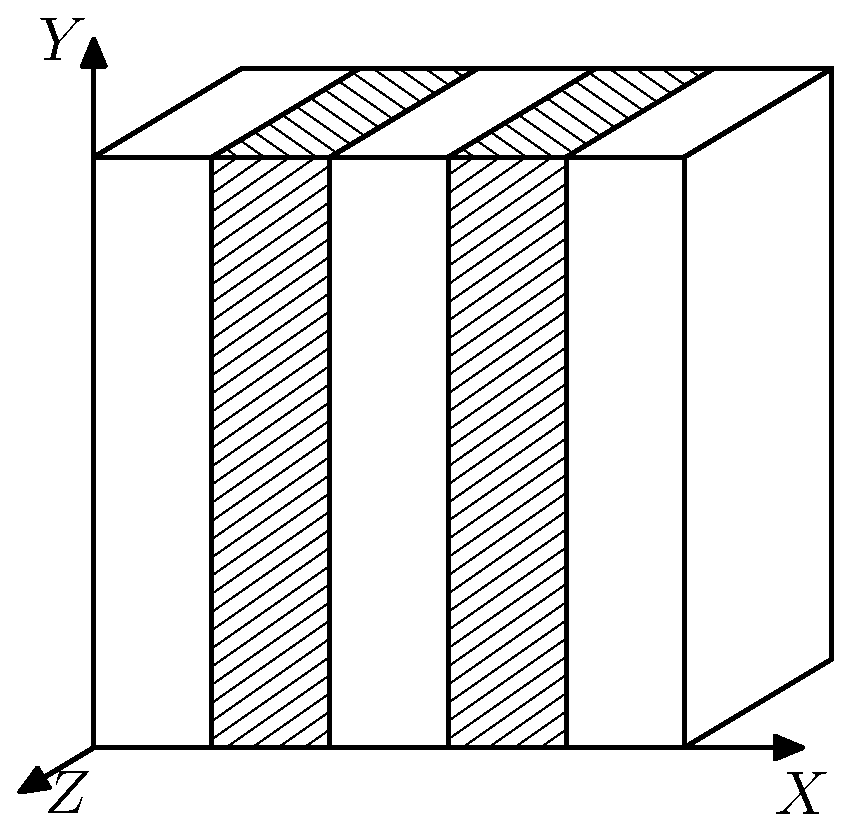
\includegraphics [scale=0.5] {one_period}
    \caption{1-периодчекая среда.} 
    \label{images:one_period}  
\end{figure}
% \begin{figure}[h]
%     \def\svgwidth{1.5\textwidth}%
%     \resizebox{\textwidth}{!}{%
%         \input{num1.tex}%
%     }
%     \caption{Test with ``figure'' environment.}
% \end{figure}

2-периодические коомпозитные материалы (армированные) (рис. 
\ref{images:two_period}
).
Физические свойства изменяются периодически вдоль двух направлений (на рис. 
\ref{images:two_period} $Ox$
и 
$Oy$
).  Вдоль третьего направления 
($Oz$) 
физические свойства не изменяются. 

\begin{equation}
    \begin{array}{ccc}
    \vec{a}_x = \left(\begin{array}{c}h_x\\0\\0\end{array}\right) & 
    \vec{a}_y = \left(\begin{array}{c}0\\h_y\\0\end{array}\right) & 
    \vec{a}_z = \left(\begin{array}{c}0\\0\\0\end{array}\right)
    \end{array}
\end{equation}

\begin{figure} [ht] 
    \center
    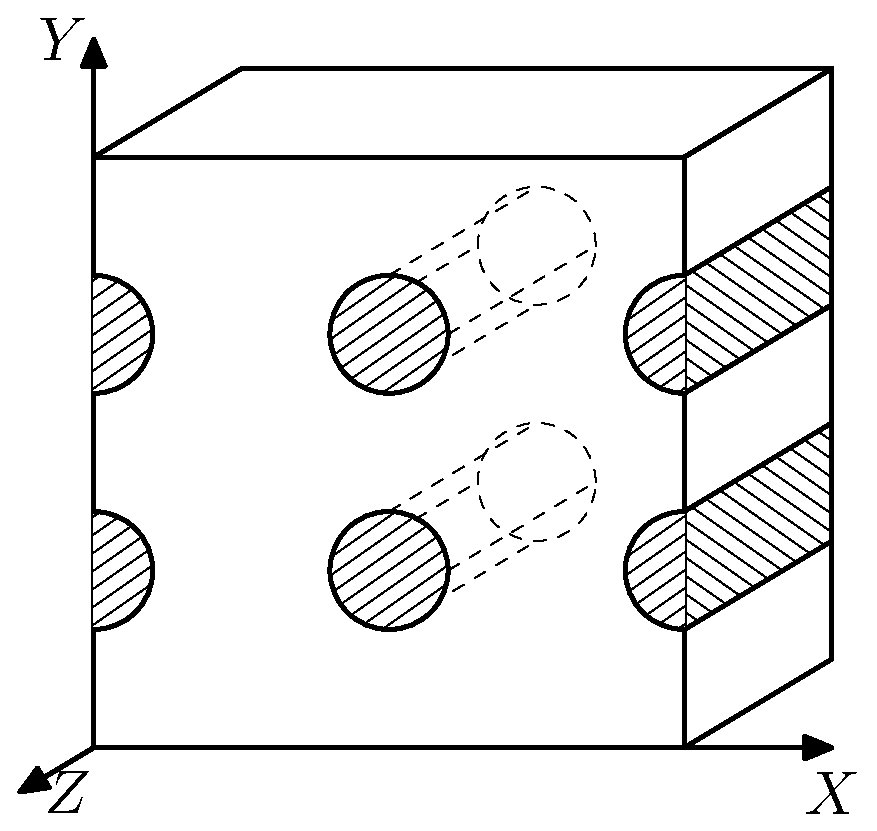
\includegraphics [scale=0.5] {images/two_period}
    \caption{2-периодчекая среда.} 
    \label{images:two_period}  
\end{figure}

3-периодические коомпозитные материалы (рис. 
\ref{images:three_period}
).  Физические свойства изменяются периодически вдоль всех трёх направлений.

\begin{equation}
    \begin{array}{ccc}
    \vec{a}_x = \left(\begin{array}{c}h_x\\0\\0\end{array}\right) & 
    \vec{a}_y = \left(\begin{array}{c}0\\h_y\\0\end{array}\right) & 
    \vec{a}_z = \left(\begin{array}{c}0\\0\\h_z\end{array}\right)
    \end{array}
\end{equation}

\begin{figure} [ht] 
    \center
    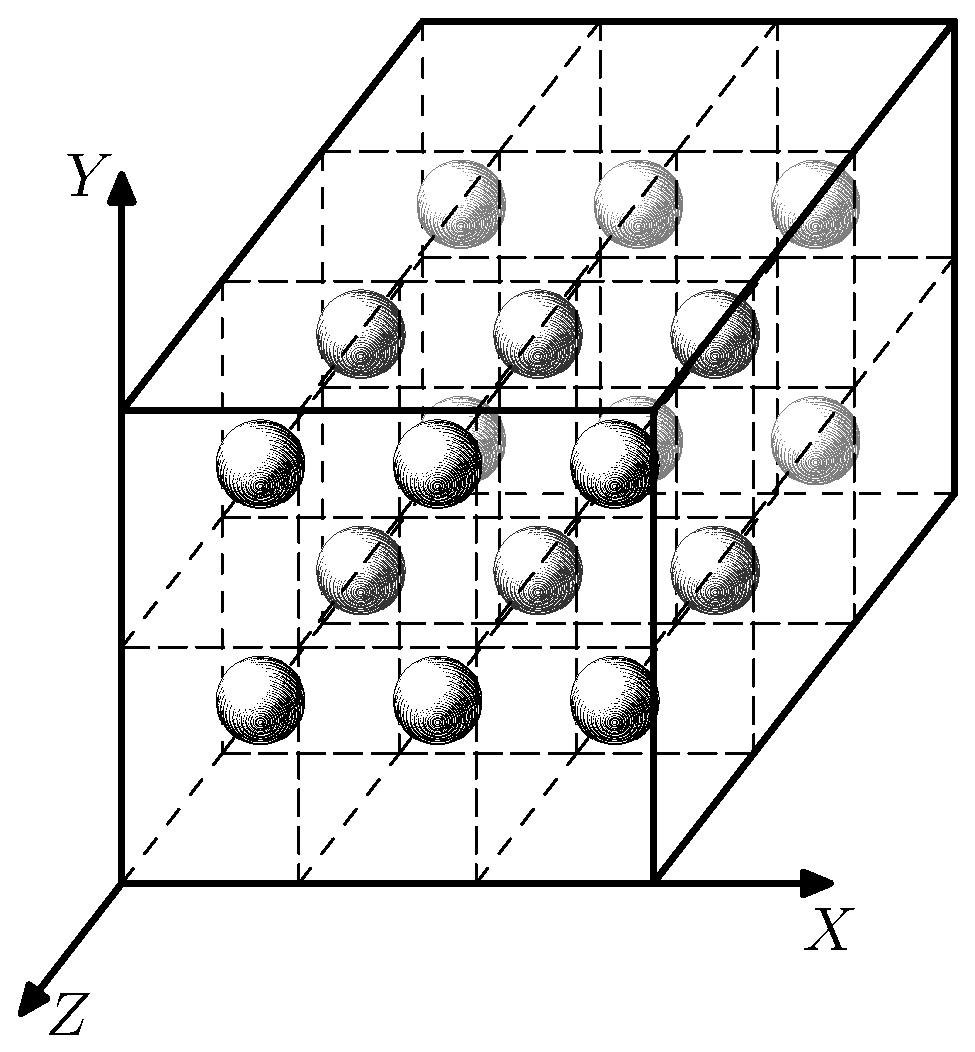
\includegraphics [scale=0.5] {images/three_period}
    \caption{3-периодчекая среда.} 
    \label{images:three_period}  
\end{figure}

Область в которой определяющие соотношения 
\ref{eq:BasicDefRelations}
непрерывны по координате будем называть компонентом композита.
Композит может иметь два и более компонента. 
Если композит двухкомпонентный, то один из компонентом можно называть связующим (матрицей), а другой включениями (в случае армированного композита арматурой, волокнами).

Функция
$\mathfrak{a}$,
входящая в правую часть соотношения
\ref{eq:BasicDefRelations},
непрерывна во всей области и не терпит разыв на границе раздела сред. 
В случае задачи упругости это соответствует идеальному контакту сред, входящих в состав композита, деформации не терпят разрыв на грнанице раздела сред.

Материльные функции изменяются с периодом порядка величины
$ \varepsilon \ll 1 $
. В таком случае при решении задачи напрямую численным методом придётся сильно измельчать сетку,
чотбы хотя бы несколько узлов попали на одно включение. 


\section{Формулировка задачи}\label{sec:ch1/sec2}

\section{Обзор методов}\label{sec:ch1/sec3}

\section{Разбор асимптотики}\label{sec:ch1/sec4}

\section{Асимптотическое расщепление задачи теплопроводности}\label{sec:ch1/sec5}

\begin{center}
    \Huge{Асимптотическое расщепление задачи теплопроводности, начало}
\end{center}

\section{Введение}

Рассмотрим тело вырезанное из 3-периодисческой твердотельной среды (рис ) на которое действуют какие-либо тепловые нагрузки, тогда внутри тела должно выполнятся
стциотнарное уравнение теплового равновесия:
\begin{equation}
    \label{heat_equation}
    \frac{\partial q_x}{\partial x} + \frac{\partial q_y}{\partial y} + \frac{\partial q_z}{\partial z} = -Q
\end{equation}
где 
$Q$
- обьемные источниеки тепла, 
$q_\alpha$ 
- компоненты вектора теплового потока внутри среды.
На границеперехода от одной упругой среды к другой должны быть неперывны тепловой поток и температура:

\begin{equation}
    \label{hc_eq2}
    \left[ q_\alpha \right] = 0, \left[ T \right] = 0, \alpha \in \{ x,y,z \}
\end{equation}

Внутри среды возникает анизатропный закон Фурье, содержащий 6 независимых коэффициенотв теплопроводности 
$\lambda_{\alpha \beta}$:
\begin{equation}
    \label{hc_law}
    q_{\alpha} = - \sum_{\beta \in \{x,y,z\}}\lambda_{\alpha \beta}\frac{\partial T}{\partial \beta}, \alpha \in \{x,y,z\}
\end{equation}

Пусть 
$h$
- линейный размер пвериодической ячейки, 
$L$
- характерный размер тела, 
$T_{\ast}$ $\lambda_{\ast}$ 
- характерные значения температуры и коэффициента 
теплопроводности. Перрейдем к безразмерным переменным и функциям, для простоты не меняя обозначения:
\begin{equation}
x \leftrightarrow \frac{x}{L}, 
y \leftrightarrow \frac{y}{L}, 
z \leftrightarrow \frac{z}{L},
T \leftrightarrow \frac{T}{T_{\ast}},
\lambda_{\alpha \beta} \leftrightarrow \frac{\lambda_{\alpha \beta}}{\lambda_{\ast}},
q \leftrightarrow \frac{q}{q},
Q \leftrightarrow \frac{Q}{q}
\end{equation}

В дальнейщем будем считать, что отношение размера периодической ячейки упругой среды к характерному размеру тела является малым 
параметром и обозначается буквой 
$\varepsilon$:
\begin{equation}
    \varepsilon = \frac{h}{L} \ll 1
\end{equation}

Тогда уравнение 
(\ref{heat_equation}) 
и закон теплопроводности 
(\ref{hc_law}) 
в новых переменных примут вид:
\begin{equation}
    \frac{\partial q_x}{\partial x}\varepsilon + \frac{\partial q_y}{\partial y}\varepsilon + \frac{\partial q_z}{\partial z}\varepsilon = -Q
\end{equation}

\begin{equation}
    q_{\alpha} = \sum_{\beta \in \{x,y,z\}}\lambda_{\alpha\beta} \frac{\partial T}{\partial \beta}\varepsilon, \alpha \in \{x,y,z\}
\end{equation}

Внутри каждой периядической ячейке вводятся свои ячейковые координаты 
$\xi_x$, $\xi_y$, $\xi_z$:
\begin{equation}
    \label{cell_coor}
    \alpha=\alpha_i + \xi_{\alpha}\varepsilon, \; \xi_{\alpha} \in \{0,1\}, \; \alpha \in \{x,y,z\}
\end{equation}

Где - 
$\alpha_i$ 
координаты i-ой периодической ячейки. Коэффициэты теплопроводности 3-периодической среды являются функциями только ячейковых координат 
$\xi$:
\begin{equation}
    \lambda_{\alpha \beta} = \lambda_{\alpha \beta}(\xi_x, \xi_y, \xi_z)
\end{equation}

С учетом равеннства 
(\ref{cell_coor}) 
оператор частрого дифференциирования принимает вид:
\begin{equation}
    \label{diff_oper}
    \frac{\partial}{\partial \alpha}=\frac{\partial}{\partial \alpha} + \frac{1}{\varepsilon}\frac{\partial}{\partial \xi_{\alpha}}, \; \alpha \in \{x,y,z\}
\end{equation}

Задача 
(\ref{heat_equation})
-
(\ref{hc_law})
с учетом формулы 
(\ref{diff_oper})
принимает втд:
\begin{equation}
    \label{heat_equation_epsilon}
    \frac{q_x}{\partial x}\varepsilon+
    \frac{q_y}{\partial y}\varepsilon+
    \frac{q_z}{\partial z}\varepsilon+
    \frac{q_x}{\partial \xi_x}+
    \frac{q_y}{\partial \xi_y}+
    \frac{q_z}{\partial \xi_z}=
    -Q
\end{equation}

Условия на границе перехода от одной упругой среды к другой:
\begin{equation}
    \left[ q_\alpha \right] = 0, \left[ T \right] = 0, \alpha \in \{ x,y,z \}
\end{equation}

Закон теплопролводности:
\begin{equation}
    \label{hc_law_epsilon}
    q_{\alpha}=\sum_{\beta \in \{x,y,z\}}\lambda_{\alpha \beta}\left(\frac{\partial T}{\partial \beta}\varepsilon+\frac{\partial T}{\partial \xi_{\beta}}\right), \:
    \alpha \in \{x,y,z\}
\end{equation}

Для решения задачи 
(\ref{heat_equation_epsilon})
-
(\ref{hc_law_epsilon})
используем метод асимптотического расщепления. Для этого представим асимптотические приближения температуры и компонент теплового потока,
как суммы частных дифференциальных операторов, коэффициенты которых зависят только от ячейковых переменных:

\begin{equation}
    \label{asimp_T_q}
    \begin{aligned}
        T^{(n)} = 
        \sum^n_{k=0} \left( \sum_{k_x+k_y+k_z=k} \Psi^{\overline{k}}(\overline{\xi})  
        \frac{\partial^kT^{(n)}_0}{\partial \overline{r}^{\overline{k}}}\varepsilon^k \right) ,
        \\
        q^{(n)}_{\alpha} = 
        \sum^n_{k=0} \left( \sum_{k_x+k_y+k_z=k} K^{\overline{k}}_{\alpha}(\overline{\xi})  
        \frac{\partial^kT^{(n)}_0}{\partial \overline{r}^{\overline{k}}}\varepsilon^k \right)
    \end{aligned}
\end{equation}

где использованы следующие обозначения
\begin{equation}
    \begin{gathered}
        \partial \overline{r}^{\overline{k}} = \partial x^k \partial y^k \partial z^k, \;
        \overline{k} = (k_x,k_y,k_z) = k_x \overline{e}_x+k_y \overline{e}_y+k_z \overline{e}_z,
        \\
        |\overline{k}| = k = k_x+k_y+k_z, \; \overline{r} = (x.y.z) = x \overline{e}_x + y \overline{e}_y + z \overline{e}_z,
        \\
        \overline{\xi} = \left( \xi_x + \xi_y, + \xi_z \right) = \xi_x \overline{e}_x + \xi_y \overline{e}_y + \xi_z \overline{e}_z
    \end{gathered}
\end{equation}


Будем считать, что объёмные силы имеют расщепленный вид относительно переменных среды макросреды и ячейковых переменных:

\begin{equation}
    \label{volum_force}
    Q \left( \overline{r}, \overline{\xi} \right) = \kappa \left( \overline{\xi} \right) Q_0 \left( \overline{r} \right)
\end{equation}

причем равнодействующие сомножителя, зависят от быстрых переменных, на ячейке равняется еденице:

\begin{equation}
    \label{integ_vf}
    \int_0^1 \int_0^1 \int_0^1 \kappa \left( \overline{\xi} \right) d\xi_x d\xi_y d\xi_z = 1
\end{equation}

В дальнейшем интнграл от какой-то величины по ячейковым переменным, взятых по всей ячейке, будем называть усреднением этой величины по ячейке и обозначать:

\begin{equation}
    \left< \_ \right> = \int_0^1 \int_0^1 \int_0^1 \_ d\xi_x d\xi_y d\xi_z = 1
\end{equation}

А из равенства 
(\ref{volum_force})
-
(\ref{integ_vf})
следует что величина имеет физический смысл - это среднее значение теплового источника, т.е. 
это тепловой источник макросреды:
\begin{equation}
    Q_0 \left( \overline{r} \right) = \left<  Q \left( \overline{r}, \overline{\xi} \right) \right>
\end{equation}

Далее введем предположение, что тепловой источник макросреды также может быть разложен в степень дифференциальных операторов:
\begin{equation}
    \label{asimp_Q}
    Q_0 \left( \overline{r} \right) = \sum^n_{k=0} \left( \sum_{k_x+k_y+k_z=k} \Lambda^{ \overline{k}} \frac{\partial^k T^{(n)}_0}{\partial \overline{r}^{ \overline{k}}} \right)
    , \; \alpha \in \{x,y,z\}
\end{equation}

где 
$\Lambda^{ \overline{k}}$ 
- некоторые константы с векторним вкрхним индексом, которые будут определены позднее.

Подставим формулы 
(\ref{asimp_T_q})
,
(\ref{volum_force})
и 
(\ref{asimp_Q})
в равенства 
(\ref{heat_equation_epsilon})
-
(\ref{hc_law_epsilon}) и 
приравняем коэффициенты при одинакрвых дифференциальных операторах, получим систему уравнений в частных проиезводных
на неизвестные ячейковые функции:
уравнения теплового равновесия ячейки

\begin{equation}
    \label{eq_eq_cell}
    \frac{\partial K^{ \overline{k}}_x}{\partial \xi_x}+
    \frac{\partial K^{ \overline{k}}_y}{\partial \xi_y}+
    \frac{\partial K^{ \overline{k}}_z}{\partial \xi_z}+
    K^{ \overline{k}- \overline{e}_x}_x+
    K^{ \overline{k}- \overline{e}_y}_y+
    K^{ \overline{k}- \overline{e}_z}_z=
    -\kappa \left( \overline{\xi} \right) \Lambda^{ \overline{k}}
\end{equation}

закон теплопроводности внутри периодической ячейки

\begin{equation}
    K^{ \overline{k}}_{\alpha} \left( \xi \right) = 
    - \sum_{\beta \in \{x,y,z\}} \lambda_{\alpha\beta} 
    \left(  \frac{\partial \Psi^{ \overline{k}}}{\partial \xi_{\beta}} + \Psi^{ \overline{k} - \overline{e}_{\beta}}\right)
    , \; \alpha \in \{x,y,z\}
\end{equation}

условия сопряжения терловых потоков и температур внутри ячейки

\begin{equation}
    \left[  K^{ \overline{k}}_n \right] = 0, \; \left[  \Psi^{ \overline{k}}\right] = 0
\end{equation}

из условия периодичесности ячейковых функций

\begin{equation}
    \label{periodic_cell}
    \left. \Psi^{ \overline{k}} \left( \overline{\xi} \right) \right|_{\xi_{\alpha}=0} =
    \left. \Psi^{ \overline{k}} \left( \overline{\xi} \right) \right|_{\xi_{\alpha}=1}, \;
    \left. K^{ \overline{k}} \left( \overline{\xi} \right) \right|_{\xi_{\alpha}=0} =
    \left. K^{ \overline{k}} \left( \overline{\xi} \right) \right|_{\xi_{\alpha}=1}
    , \; \alpha \in \{x,y,z\}
\end{equation}

Выражение 
(\ref{eq_eq_cell})
-
(\ref{periodic_cell})
для каждого фиксированного целочисленного вектора 
$ \overline{k} $
представляют собой краевую эллиптическую задачу на нахождение 
периодических ячейковых функций 
$ \Psi^{ \overline{k}} $
. Необходимое условие разрешимости этой задачи имеет вид:

\begin{equation}
    \label{solv_cond}
    \Lambda^{ \overline{k}} = - \left< K^{ \overline{k} - \overline{e}_x}_x + K^{ \overline{k} - \overline{e}_y}_y + K^{ \overline{k} - \overline{e}_z}_z \right> 
\end{equation}

При 
$k=0$
решение задачи 
(\ref{eq_eq_cell})
-
(\ref{solv_cond})
имеет очевидное решение:

\begin{equation}
    \label{psi_one}
    \Psi^{ \overline{0}} = 1, ;\ K^{ \overline{0}}
    , \; \alpha \in \{x,y,z\}
\end{equation}

Тогда из 
(\ref{solv_cond})
следует равенство

\begin{equation}
    \label{lambda_zero}
    \Lambda^{ \overline{k}} = 0, \left| \overline{k} \right| 
\end{equation}

Равенство 
(\ref{asimp_Q})
с учетом равенста 
(\ref{lambda_zero})
имеет вид

\begin{equation}
    \label{asimp_Q_2}
    \sum^n_{k=2} \left( \sum_{k_x+k_y+k+z=k} \Lambda^{ \overline{k}} \frac{\partial^k T^{(n)_0}}{\partial \overline{r}^{ \overline{k}}} \right) =
    Q_0 \left( \overline{r} \right) 
\end{equation}

Данное равенство представляет соьбой уравнение на n-е приближение температуры макросреды 
$T^{(n)}_0$
. Уравнение представдялет собой уравнение в частных
производных, оно имеет порядок n, теория таких уравнений рассмотрена в 
\colorbox{yellow}{(ССЫЛКО!!!)}
, в частности, из нее следует, что асимптотический смысл имеет не 
все решения этого уравнения, а только часть из них, регулярно зависящая от малого параметра 
$\varepsilon$
, а это означат, что данное уравнение
имеет действительный порядок равный двум.
Формулы 
(\ref{asimp_T_q})
с учетом равенств 
(\ref{psi_one})
принимают вид

\begin{equation}
    \label{asimp_T_q_2}
    \begin{aligned}
        T^{(n)} = T^{(n)}_0 +
        \sum^n_{k=1} \left( \sum_{k_x+k_y+k_z=k} \Psi^{\overline{k}}(\overline{\xi})  
        \frac{\partial^kT^{(n)}_0}{\partial \overline{r}^{\overline{k}}}\varepsilon^k \right) ,
        \\
        q^{(n)}_{\alpha} = 
        \sum^n_{k=1} \left( \sum_{k_x+k_y+k_z=k} K^{\overline{k}}_{\alpha}(\overline{\xi})  
        \frac{\partial^kT^{(n)}_0}{\partial \overline{r}^{\overline{k}}}\varepsilon^k \right)
    \end{aligned}
\end{equation}

эти равенства являются формулами для вычисления температуры и компонент теплового потока в периодической среде на основе решения уравнения 
(\ref{asimp_Q_2})
и краевых задач 
(\ref{eq_eq_cell})
-
(\ref{solv_cond})
. Величина 
$T^{(n)}_0$ 
имеет физический смысл, она является средним значением распределения температуры на ячейке, т.е. эта величина является 
температурой однородной макросреды:

\begin{equation}
    T^{(n)}_0 = \left< T^{(n)} \left( \overline{r}, \overline{\xi} \right)  \right> 
\end{equation}

Наибольший интерес в любой асимптотической теории представляют самые первые приближения, в данном случае это 
$n=2$
. Усреднми вектор теплового потока 
(\ref{asimp_T_q_2})
при 
$n=2$
и рассмотрим его первое приближение, в дальнейшем верхние индексы, указывающие на номера асимптотического приближения, опускаем:

\begin{equation}
    \label{asimp_q_n_2}
    \widetilde{q}_{\alpha} = 
    \sum_{\phi \in \{x,y,z\}} \left< K^{ \overline{e}_{\phi}}_{\alpha} \left( \overline{\xi} \right)  \right> 
    \frac{\partial T_0}{\partial \phi} \varepsilon
    , \; \alpha \in \{x,y,z\}
\end{equation}

Можно показать, что этот вектор удовлетворяет следующему уравнению теплового баланса:

\begin{equation}
    \label{eq_eq_meta}
    \frac{\partial \widetilde{q}_x}{\partial x}\varepsilon + 
    \frac{\partial \widetilde{q}_y}{\partial y}\varepsilon + 
    \frac{\partial \widetilde{q}_z}{\partial z}\varepsilon = -Q
\end{equation}

В уравнении 
(\ref{eq_eq_meta}) 
спрва стоит тепловой источник макросреды, вектор 
$ \widetilde{q}_{\alpha}$ 
зависит только от переменных макросреды, поэтому можно считать, 
что вектор 
$ \widetilde{q}_{\alpha}$ 
- это вектор теплового потока в однородной макросреде, а уравнение 
(\ref{asimp_q_n_2}) 
- это закон теполопроводности в макросреде, это уравнение может быть переписано
в виде:

\begin{equation}
    \widetilde{q}_{\alpha} = - \sum_{ \phi \in \{x,y,z\} } \widetilde{\lambda}_{\alpha\phi} \frac{\partial T_0}{\partial \phi} \varepsilon
\end{equation}

где 
$ \widetilde{\lambda}_{\alpha\phi}$ 
- коэффициент теплопроводности макросреды, они рассчитываются на омнове решений данных ячейковых краевых задач:

\begin{equation}
    \widetilde{\lambda}_{\alpha\phi} = - \left< K^{ \overline{e}_{\phi}}_{\alpha} \left( \overline{\xi} \right) \right> 
    , \; \alpha,\phi \in \{x,y,z\} 
\end{equation}

Для расчета коэффициентов теплопроводности макросреды необходимо решить следующие три краевые задачи на ячейке:

урввнение
\begin{equation}
    \frac{K^{ \overline{e}_{\phi}}_x}{\partial \xi_x} +
    \frac{K^{ \overline{e}_{\phi}}_y}{\partial \xi_y} +
    \frac{K^{ \overline{e}_{\phi}}_z}{\partial \xi_z} = 0,
    \phi \in \{x,y,z\} 
\end{equation}

закон теплопроводности на ячейке
\begin{equation}
    K^{ \overline{e}_{\phi}}_{\alpha} \left( \overline{\xi} \right) =
    - \sum_{ \beta \in \{x,y,z\} } \lambda_{\alpha\beta}
    \left( \frac{\partial \Psi^{ \overline{e}_{\phi}}}{\partial \xi_{\beta}} + \delta^{\phi}_{\beta} \right) 
\end{equation}

условие непрерывности на границах раздела матрицы и включений
\begin{equation}
    \left[  K^{ \overline{e}_{\phi}}_n \right] = 0, \; \left[  \Psi^{ \overline{e}_{\phi}}\right] = 0
    , \; \phi \in \{x,y,z\}
\end{equation}

условие периодичности ячейковых функций
\begin{equation}
    \begin{gathered}
    \left. \Psi^{ \overline{e}_{\phi}} \left( \overline{\xi} \right) \right|_{\xi_{\alpha}=0} =
    \left. \Psi^{ \overline{e}_{\phi}} \left( \overline{\xi} \right) \right|_{\xi_{\alpha}=1}, \;
    \left. K^{ \overline{e}_{\phi}} \left( \overline{\xi} \right) \right|_{\xi_{\alpha}=0} =
    \left. K^{ \overline{e}_{\phi}} \left( \overline{\xi} \right) \right|_{\xi_{\alpha}=1},
    \\
    \alpha,\phi \in \{x,y,z\}
    \end{gathered}
\end{equation}



\section{Асимптотическое расщепление задачи упругости}\label{sec:ch1/sec6}

Рассмотрим тело вырезанное из 3-периодической среды, на которое действуют какиелибо нагрузки, тогда внутри тела должны ваполнятся уравнения
равновесия:

\begin{equation}
    \label{elhp:eq1}
    \frac{\partial \sigma_{\beta x}}{\partial x} +
    \frac{\partial \sigma_{\beta y}}{\partial y} +
    \frac{\partial \sigma_{\beta z}}{\partial z} +
    F_{\beta} = 0,
    \beta \in \{x,y,z\} 
\end{equation}

гда 
$F_{\beta}$ 
- обьёмные силы. На границе перехода от одной упругой чреды к другой должны быть непрорывны перемещения и контактные напряжения:

\begin{equation}
    \label{elhp:eq2}
    \left[ \sigma_{\beta n} \right] = 0, \left[ u_{\beta} \right] = 0, \beta \in \{x,y,z\} 
\end{equation}

где $\sigma_{\beta n}$ -  контактные напряжения, которые по определению вычисляются по следующей формуле

\begin{equation}
    \label{elhp:eq3}
    \sigma_{\beta n} = 
    \sigma_{\beta x} n_x +
    \sigma_{\beta y} n_y +
    \sigma_{\beta z} n_z
\end{equation}

Считаем, что каждый материал является анизотропно уругим. Закон Дюамеля-Неймона зависимости напряжений от температуры в общем случае для
каждого материала содержит 21 независимую упрегую константц 
$E_{\gamma\beta\phi\psi}$ 
и 6 констант тензора линейного температурного 
расширения 
$\alpha_{\phi\psi}$ 
и имеет вид (\colorbox{yellow}{ССЫЛКО!!!})

\begin{equation}
    \label{elhp:eq4}
    \sigma_{\gamma \beta} = \sum_{ \phi, \psi \in \{x,y,z\} } E_{\gamma\beta\phi\psi} 
    \left( e_{\phi\psi} - \alpha_{\phi\psi}T \right) \gamma,\beta \in \{x,y,z\} 
\end{equation}

Компоненты тензора деформаций связаны с компонентами вектора перемещений соотношениями Коши:

\begin{equation}
    \label{elhp:eq5}
    e_{\gamma\beta} = \frac{1}{2} \left( \frac{\partial u_{\gamma}}{\partial \beta} + \frac{\partial u_{\beta}}{\partial \gamma}  \right) 
    ,\; \gamma,\beta \in \{x,y,z\} 
\end{equation}

Кроме того, к равенству 
(\ref{elhp:eq1})
-
(\ref{elhp:eq5}) 
должны быть добавлены краевые условия на границе тела. 
С учетом их, задача 
(\ref{elhp:eq1})
-
(\ref{elhp:eq5}) 
является краевой задачей, решениями 
которой явзяются перемещения, по которым их равенства 
(\ref{elhp:eq4}) 
могут быть найдены термонапряжения.

Пусть i
$ \widetilde{u} $ 
- характерное значение для перемещения 
$h_x$, $h$ 
- линейный размер периодической решетки (куба), 
$L$ 
- характерный размер тела,
$ \widetilde{E}$, $ \widetilde{T}$ 
- характерное среднее значение модуля Юнга и изменения температуры соответственно. Перейдём к безразмерным переменным и функциям,
для простоты не меняя их обозначения:

\begin{equation}
    \label{elhp:eq6}
    \begin{aligned}
        x \leftrightarrow \frac{x}{L}, 
        y \leftrightarrow \frac{y}{L}, 
        z \leftrightarrow \frac{z}{L},
        u_{\gamma} \leftrightarrow \frac{u_{\gamma}}{h},
        E_{\gamma\beta\phi\psi} \leftrightarrow \frac{E_{\gamma\beta\phi\psi}}{ \widetilde{E}},
        \\
        \sigma_{\gamma\beta}\leftrightarrow \frac{\sigma_{\gamma\beta}}{ \widetilde{E}},
        q_{\gamma} \leftrightarrow \frac{q_{\gamma}}{ \widetilde{E}},
        T \leftrightarrow \frac{T}{ \widetilde{T}},
        \alpha_{\phi\psi} \leftrightarrow \alpha_{\phi\psi} \widetilde{T},
        \widetilde{F}_{\gamma} \leftrightarrow \frac{F_{\gamma}}{ \widetilde{E}}
    \end{aligned}
\end{equation}

В дальнейшем будем считать, что отношение размера периодической ячейки упругой среды к характерному размеру тела является малым параметром
и обознчается буквой 
$\varepsilon$:

\begin{equation}
    \label{elhp:eq7}
    \varepsilon = \frac{h}{L} \ll 1
\end{equation}

Тогда уравнения 
(\ref{elhp:eq1})
в новых переменных примут вид

\begin{equation}
    \label{elhp:eq8}
    \frac{\partial \sigma_{\gamma x}}{\partial x}\varepsilon +
    \frac{\partial \sigma_{\gamma y}}{\partial y}\varepsilon +
    \frac{\partial \sigma_{\gamma z}}{\partial z}\varepsilon +
    F_{\alpha} = 0
\end{equation}

Равенства 
(\ref{elhp:eq2})
-
(\ref{elhp:eq4})
останутся без изменений, а выражение 
(\ref{elhp:eq5})
примет вид

\begin{equation}
    \label{elhp:eq9}
    e_{\gamma\beta} = \frac{1}{2}
    \left( \frac{\partial u_{\gamma}}{\partial \beta} \varepsilon \frac{\partial u_{\beta}}{\partial \gamma} \varepsilon \right) 
\end{equation}

Введение двух масштабов моделирования. Согласно основной идее многомасштабного метода (\colorbox{yellow}{ССЫЛКО!!!}) внутри каждой периодической ячецки положение
точки однозначно описывается тремя безразмерными координатами 
$\xi_x, \xi_y, \xi_z$
, с помощью формул

\begin{equation}
    \label{elhp:eq10}
    x = x_i + \xi_x \varepsilon ,\;
    y = y_i + \xi_y \varepsilon ,\;
    z = z_i + \xi_z \varepsilon ,\;
    \xi_x,\xi_y,\xi_z \in \{x,y,z\} 
\end{equation}

где
$x_i, y_i, z_i$ 
- координаты i-го периодического куба. Координаты  
$\xi_x, \xi_y, \xi_z$ 
будем называть ячейквыми в противоположность пространственным 
координатам 
$x,y,z$
, в то время когда ячейковые координаты изменяются на единицу, соответствующие им простренственные меняются на малую величину 
$\varepsilon$
, как это следует из формулы 
(\ref{elhp:eq10})
.

Упругие и термоупругие характеристики 3-периодической среды будем считать зависящими только от ячейковых координат 
$\varepsilon$:

\begin{equation}
    \label{elhp:eq11}
    E_{\gamma\beta\phi\psi} = 
    E_{\gamma\beta\phi\psi} 
    \left( \overline{\xi} \right) 
    ,\;
    \alpha_{\phi\psi} = 
    \alpha_{\phi\psi}
    \left( \overline{\xi} \right) 
\end{equation}

Хотя солгасно формулам 
(\ref{elhp:eq10})
координаты i
$ \left( x,y,z \right) $ 
и 
$ \left( \xi_x, \xi_y, \xi_z \right) $ 
являются зависимыми, в дальнейшем
будем формально считать, что все неизвестные функции
одновременно зависят как от ячейковых координат 
$ \left( \xi_x, \xi_y, \xi_z \right) $
, так и от координат 
$ \left( x,y,z \right) $

\begin{equation}
    \label{elhp:eq13}
    u_{\gamma} =
    u_{\gamma}
    \left( \overline{\xi}, \overline{r} \right) 
    ,\;
    \sigma_{\gamma\beta} = 
    \sigma_{\gamma\beta}
    \left( \overline{\xi}, \overline{r} \right) 
    ,\;
    \gamma,\beta \in \{x,y,z\} 
\end{equation}

при этом фломулы 
(\ref{elhp:eq10})
продолжют остраваться справедливыми. Координаты 
$ \left( x,y,z \right) $ 
в дальнейшем будем называть макрокоординатами (макропеременными)
так как они однозначным образом фиксируют положение макросреды, которая будет введена в дальнейшем. Потребуем также условия периодичности неизвестных
функций по ячейковым перемещениям и напряжениям:

\begin{equation}
    \label{elhp:eq14}
    \begin{gathered}
    u_{\beta} \left. \left( \overline{\xi}, \overline{r} \right)  \right|_{\xi_{\gamma}=0} =
    u_{\beta} \left. \left( \overline{\xi}, \overline{r} \right)  \right|_{\xi_{\gamma}=1} 
    ,\;
    \sigma_{\gamma\beta} \left. \left( \overline{\xi}, \overline{r} \right)  \right|_{\xi_{\gamma}=0} =
    \sigma_{\gamma\beta} \left. \left( \overline{\xi}, \overline{r} \right)  \right|_{\xi_{\gamma}=1} 
    ,
    \\
    \gamma,\beta \in \{x,y,z\} 
    \end{gathered}
\end{equation}

С учеотом равенства 
(\ref{elhp:eq10})
оператор частного дифференцирования принимает вид диыыеренциирования и по ячейковым переменным и по макропеременнвм (\colorbox{yellow}{ССЫЛКО!!!}):

\begin{equation}
    \label{elhp:eq15}
    \frac{\partial }{\partial \gamma} = \frac{\partial }{\partial \gamma} + \frac{1}{\varepsilon} \frac{\partial \xi_{\varepsilon}}{\partial } 
\end{equation}

Уравнения 
(\ref{elhp:eq8})
, 
(\ref{elhp:eq3})
-
(\ref{elhp:eq5})
, 
(\ref{elhp:eq10})
с учетом формулы 
(\ref{elhp:eq15})
для диференциального оператора принимают вид

\begin{equation}
    \label{elhp:eq16}
    \frac{\partial \sigma_{\gamma x}}{\partial x} \varepsilon + 
    \frac{\partial \sigma_{\gamma y}}{\partial y} \varepsilon + 
    \frac{\partial \sigma_{\gamma z}}{\partial z} \varepsilon + 
    \frac{\partial \sigma_{\gamma x}}{\partial \xi_x} \varepsilon + 
    \frac{\partial \sigma_{\gamma y}}{\partial \xi_y} \varepsilon + 
    \frac{\partial \sigma_{\gamma z}}{\partial \xi_z} \varepsilon + 
    F_{\gamma} = 0
\end{equation}

условие на границе от одной упругой среды к другой:

\begin{equation}
    \label{elhp:eq17}
    \left[ \sigma_{\gamma n} \right] = 0, \; \left[ u_{\gamma} \right], \; \gamma,\beta \in \{x,y,z\} 
\end{equation}

закон Дюамеля-Неймона:

\begin{equation}
    \label{elhp:eq18}
    \sigma_{\gamma\beta} = \sum_{ \phi\psi \in \{x,y,z\} }
    E_{\gamma\beta\phi\psi} 
    \left( e_{\phi\psi} - \alpha_{\phi\psi}T \right) 
    , \;
    \gamma,\beta \in \{x,y,z\} 
\end{equation}

формулы для компонента тензора деформаций:

\begin{equation}
    \label{elhp:eq19}
    e_{\gamma\beta} = \frac{1}{2}
    \left( 
        \frac{\partial u_{\gamma}}{\partial \beta} \varepsilon +
        \frac{\partial u_{\gamma}}{\partial \beta} \varepsilon +
        \frac{\partial u_{\gamma}}{\partial \xi_{\beta}} +
        \frac{\partial u_{\gamma}}{\partial \xi_{\beta}}
    \right) 
    , \;
    \gamma,\beta \in \{x,y,z\} 
\end{equation}

Кроме того, к уравнениям 
(\ref{elhp:eq15})
-
(\ref{elhp:eq19})
должны быть добавлены краевые условия на кганице тела.
Далее будем считать, что законы ремпределения температуры и обэёмных сил по объйму среды имеют расщепленый вид относительно  медленных и быстрых
переменных:

\begin{equation}
    \label{elhp:eq20}
    T \left( \overline{r}, \overline{\xi} \right) = \Psi \left( \overline{\xi}  \right) T_0 \left( \overline{r}  \right) 
    , \;
    F_{\gamma} \left( \overline{r}, \overline{\xi} \right) = q_{\gamma} \left( \overline{\xi}  \right) f_{\gamma} \left( \overline{r}  \right) 
\end{equation}

причем интеграл сомножтеле, зависящих от быстрых переменных, по объёму периодический ячейки равняется единице:

\begin{equation}
    \label{elhp:eq21}
    \left< \Psi \left( \overline{\xi}  \right)  \right> = 1
    ,\;
    \left< q_{\gamma} \left( \overline{\xi}  \right)  \right> = 1
\end{equation}

Условие 
(\ref{elhp:eq21})
является нормировочным. А из равенств 
(\ref{elhp:eq19})
-
(\ref{elhp:eq21})
следует, функция 
$T_0 \left(  \overline{r} \right) $ 
является средней температурой в 
ячейке периодичности, а 
$f_{_gamma} \left( \overline{r}  \right) $
- средней объёмной силой, действующей на ячейку периодичности: 

\begin{equation}
    \label{elhp:eq22}
    T_0 \left( \overline{r}  \right) = \left< T \left( \overline{r} , \overline{\xi}  \right)  \right> 
    ,\;
    f_{\gamma} \left( \overline{r}  \right) = \left< T \left( \overline{r} , \overline{\xi}  \right)  \right> 
    ,\;
    \gamma \in \{x,y,z\} 
\end{equation}

Метод асимптотического расщепления. В соответствии с общей идеей метода асимптотического расщепления ищем перемещения и напряжения в виде
конечных сумм дифференнциальных операторов по макропеременным, а среднюю температуру и средние объёмные силы также представляем в виде суммы 
дифференциированных операторов по макропеременным, а среднюю температуру и средние объёмные силы также представляем в виде сумм дифференциальных 
операторов по макропеременным, 
$n$
- номер асимаптотического приближения:

\begin{equation}
    \label{elhp:eq23}
    \left( u_{\gamma} \right)^{(n)} =
    v_{\gamma}^{(n)} +
    \sum_{ \omega \in \{x,y,z\} } \sum_{k=1}^{n+1}
    \left( 
    \sum_{k_x+k_y+k_z = k} 
    \left( U_{\gamma}^{v_{\theta}} \right)^{ \overline{k} } 
    \frac{\partial^k v_{\theta}^{(n)}}{\partial \overline{r}^{ \overline{k}  } } 
    \varepsilon^k
\right) 
,\;
\gamma \in \{x,y,z\} 
\end{equation}

\begin{equation}
    \label{elhp:eq24}
    \left( \sigma_{\gamma\beta} \right)^{(n)} =
    \sum_{ \omega \in \{x,y,z\} } \sum_{k=1}^{n+1}
    \left( 
    \sum_{k_x+k_y+k_z = k} 
    \left( \tau_{ \gamma\beta}^{v_{\theta}} \right)^{ \overline{k} }
    \frac{\partial^k v_{\theta}^{(n)}}{\partial \overline{r}^{ \overline{k}  } } 
    \varepsilon^k
    \right) 
,\;
    \gamma,\beta \in \{x,y,z\} 
\end{equation}

\begin{equation}
    \label{elhp:eq25}
    T_0 \left( \overline{r}  \right) =
    \sum_{ \omega \in \{x,y,z\} } 
    \left( 
        \sum_{k=1}^{n}
        A_{v_{\theta}}^{ \overline{k} }
        \frac{\partial^k v_{\theta}^{(n)}}{\partial \overline{r}^{ \overline{k}  } } 
        \varepsilon^k
    \right) 
\end{equation}

\begin{equation}
    \label{elhp:eq26}
    f_{ \gamma} \left( \overline{r}  \right) =
    \sum_{ \omega \in \{x,y,z\} } \sum_{k=2}^{n+1}
    \left( 
    \sum_{k_x+k_y+k_z = k} 
    \left( B_{\gamma}^{v_{\theta}} \right)^{ \overline{k} } 
    \frac{\partial^k v_{\theta}^{(n)}}{\partial \overline{r}^{ \overline{k}  } } 
    \varepsilon^k
\right) 
,\;
\gamma \in \{x,y,z\} 
\end{equation}


где функции 
$v_{ \gamma}^{(n)}$ 
зависят от макропеременных и поопределению равняются осреднению реальных перемещений 
$ \left(  u_{ \gamma} \right)^{(n)} $ 
по периодической ячейке:

\begin{equation}
    \label{elhp:eq27}
    v_{ \gamma}^{(n)} = \left< \left( u_{ \gamma}^{(n)} \right)  \right> 
\end{equation}

В формулах 
(\ref{elhp:eq23})
-
(\ref{elhp:eq24})
кохффициенты при степенях дифференциальных операторов по макроперемещениым зависят только от ячейковых переменных, 
поэтому их называют ячейковыми функсциями. Соответственно и метод ассимптотического расщепления применительно к задачам такого типа
называются меотдом ячейковых функций. В формулах 
(\ref{elhp:eq25})
-
(\ref{elhp:eq26})
коэффициенты являются неизвестными константами. Для рещения краевой задачи

(\ref{elhp:eq16})
-
(\ref{elhp:eq19})
достаточно подставить в нее равенмтва 
(\ref{elhp:eq23})
-
(\ref{elhp:eq26})
, затем собрать подобные и приравнять коэффициенты при дифференциальных операторах 
нулю, в итоге получается система краевых рекурентных задач на неизвестных ячейковые функции вектора перемещений и тензора напряжений:

\begin{equation}
    \label{elhp:eq28}
    \frac{\partial \left(  \tau_{ \gamma x}^{v_{\theta}}\right)^{ \overline{k} }}{\partial \xi_x} +
    \frac{\partial \left(  \tau_{ \gamma y}^{v_{\theta}}\right)^{ \overline{k} }}{\partial \xi_y} +
    \frac{\partial \left(  \tau_{ \gamma z}^{v_{\theta}}\right)^{ \overline{k} }}{\partial \xi_z} +
    \left(  \tau_{ \gamma x}^{v_{\theta}}\right)^{ \overline{k} - \overline{\epsilon_x} } +
    \left(  \tau_{ \gamma y}^{v_{\theta}}\right)^{ \overline{k} - \overline{\epsilon_y} } +
    \left(  \tau_{ \gamma z}^{v_{\theta}}\right)^{ \overline{k} - \overline{\epsilon_z} } =
    q_{\gamma} \left( \overline{\xi}  \right) \left( B_{\gamma}^{v_{\theta}} \right)^{ \overline{k} }
\end{equation}

закон термоупругости внутри ячейки

\begin{equation}
    \label{elhp:eq29}
    \begin{gathered}
    \left( \tau_{ \gamma\beta} \right)^{ \overline{k} } =
    \sum_{ \phi,\psi \in \{x,y,z\}} E_{ \gamma\beta\phi\psi}
    \\
    \left( \frac{1}{2} 
        \left( 
            \frac{\partial \left( U_{\phi}^{v_{\theta}}\right)^{ \overline{k} }}{\partial \xi_{\psi}} +
            \frac{\partial \left( U_{\psi}^{v_{\theta}}\right)^{ \overline{k} }}{\partial \xi_{\phi}} +
            \left( U_{\phi}^{v_{\theta}}\right)^{ \overline{k} - \overline{\epsilon}_{\psi}  } +
            \left( U_{\psi}^{v_{\theta}}\right)^{ \overline{k} - \overline{\epsilon}_{\phi}  }
        \right) 
        - \alpha_{\phi\psi} \Psi A_{v_{\theta}}^{ \overline{k} }
    \right) 
    \end{gathered}
\end{equation}

условия непрерывности ячейковых функций внутри ячейке на границе различных сред

\begin{equation}
    \label{elhp:eq30}
    \left[ \left( \tau_{ \gamma n}^{v_{\theta}} \right)^{ \overline{k} }  \right] = 0
    ,\;
    \left[ \left( U_{ \gamma}^{v_{\theta}} \right)^{ \overline{k} }  \right] = 0
    ,\;
    \gamma \in \{x,y,z\} 
\end{equation}

услоние периодичности ячейковых функций

\begin{equation}
    \label{elhp:eq70}
    \begin{gathered}
    \left.   
    \left( U_{\beta}^{ v_{\theta}} \right)^{ \overline{k}}
    \left( \overline{\xi}  \right) 
    \right|_{\xi_{\gamma}=0}
    =
    \left.   
    \left( U_{\beta}^{ v_{\theta}} \right)^{ \overline{k}}
    \left( \overline{\xi}  \right) 
    \right|_{\xi_{\gamma}=1}
    ,
    \\
    \left.   
    \left( \tau_{\beta\gamma}^{ v_{\theta}} \right)^{ \overline{k}}
    \left( \overline{\xi}  \right) 
    \right|_{\xi_{\gamma}=0}
    =
    \left.   
    \left( \tau_{\beta\gamma}^{ v_{\theta}} \right)^{ \overline{k}}
    \left( \overline{\xi}  \right) 
    \right|_{\xi_{\gamma}=1},
    \\
    \beta,\gamma \in \{x,y,z\} 
    \end{gathered}
\end{equation}

Из равенства 
(\ref{elhp:eq27})
следует, что к полученным равенствам следует добавить нормировки на 
ячейковые функции вектора перемещения

\begin{equation}
    \label{elhp:eq31}
    \left< \left( U_{\beta}^{v_{\theta}} \right)^{ \overline{k} } \left( \overline{\xi}  \right)   \right> = 0
    ,\;
    \gamma \in \{x,y,z\} ,\; k \ge 1
\end{equation}


Необходимое условие разрешимости краевой задачи 
(\ref{elhp:eq28})
-
(\ref{elhp:eq31})
имеет вид

\begin{equation}
    \label{elhp:eq32}
    \left( B_{\gamma}^{v_{\theta}} \right)^{ \overline{k} } =
    \left< 
    \left( \tau_{ \gamma x}^{v_{\theta}} \right)^{ \overline{k} - \overline{\epsilon_x} } +
    \left( \tau_{ \gamma y}^{v_{\theta}} \right)^{ \overline{k} - \overline{\epsilon_y} } +
    \left( \tau_{ \gamma z}^{v_{\theta}} \right)^{ \overline{k} - \overline{\epsilon_z} } 
    \right> 
    ,\;
    \gamma \in \{x,y,z\} 
\end{equation}

где треугольные скобки обозначают интегрирование по объёму перидической ячейки (по ячейковым переменным). Из формул 
(\ref{elhp:eq29})
и 
(\ref{elhp:eq32})
следует, что коэффициент 
$\left( B_{\gamma}^{v_{\theta}} \right)^{ \overline{k} }$ 
является функцией от констат 
$A_{v_{\theta}}^{ \overline{k} - \epsilon_y} ,\;A_{v_{\theta}}^{ \overline{k} - \epsilon_y} ,\;A_{v_{\theta}}^{ \overline{k} - \epsilon_z}$. 
Равенство 
(\ref{elhp:eq26})
можно рассматривать как систему уравнений в частныхпроизводных на 
макроперемещения 
$v_{\gamma}^{(n)}$:

\begin{equation}
    \label{elhp:eq33}
    \sum_{ \theta \in \{x,y,z\} } \sum_{k=2}^{n+1}
    \left( 
        \sum_{k_x+k_y+k_z = k}
        \left( B_{\gamma}^{v_{\theta}} \right)^{ \overline{k} }
        \frac{\partial^k v_{\theta}^{(n)}}{\partial \overline{r}^{ \overline{k}}}
        \varepsilon^k
    \right) 
    + f_{ \gamma} \left( \overline{r}  \right) = 0
    ,\;
    \gamma \in \{x,y,z\} 
\end{equation}

Для которой в качестве краевых условий выступаеют условия исходной краевой задачи 
(\ref{elhp:eq16})
-
(\ref{elhp:eq19})
. Равенство 
(\ref{elhp:eq25})
в общем случае не может быть выполнено 
в точности, поэтому потребуем его выполнения в смысле минимизации невязки по методу наменьших квадратов, тогда постановка задачи которую следует
решить, принимает вид.

Это задача о минимизации функционала

\begin{equation}
    \label{elhp:eq34}
    \int_V \left( 
    T_0 \left( \overline{r}  \right) - 
    \sum_{ \theta \in \{x,y,z\} } \left( 
        \sum^{n-1}_{k=1} A_{v_{\theta}}^{ \overline{k} } \frac{\partial^k v_{\theta}}{\partial \overline{r}^{ \overline{k} } } 
    \right)   \right)^2
    dV \rightarrow min
\end{equation}

при выполнении условий

\begin{equation}
    \label{elhp:eq35}
    \sum_{ \theta \in \{x,y,z\} } \sum_{k=2}^{n}
    \left( 
        \sum_{k_x+k_y+k_z = k}
        \left( B_{\gamma}^{v_{\theta}} \right)^{ \overline{k} }
        \frac{\partial^k v_{\theta}^{(n)}}{\partial \overline{r}^{ \overline{k}}}
        \varepsilon^k
    \right) 
    + f_{ \gamma} \left( \overline{r}  \right) = 0
    ,\;
    \gamma \in \{x,y,z\} 
\end{equation}

и граничных учловий на поверхности тела, где коэффициенты 
$\left( B_{\gamma}^{v_{\theta}} \right)^{ \overline{k} }$ 
вычисляются по формулам 
(\ref{elhp:eq32})
на основе решений ячейкрвых краевых задач 
(\ref{elhp:eq28})
-
(\ref{elhp:eq31})
.
Наибольший интерес в любом ассимаптотическом методе представляет первое приближение при 
$n=1$
, поэтому в дальнейшем будем рассматривать
только его.

Первое асимптотическое приближение при 
$n=1$
. В этом случае задача 
(\ref{elhp:eq34})
-
(\ref{elhp:eq35})
принимает вид:

\begin{equation}
    \label{elhp:eq36}
    \int_V \left( 
    T_0 \left( \overline{r}  \right) - 
    \sum_{ \theta \in \{x,y,z\} } \left( 
        \sum_{ \eta \in \{x,y,z\} } A_{v_{\theta}}^{ \overline{k} } \frac{\partial^k v_{\theta}}{\partial \eta } 
    \right)   \right)^2
    dV \rightarrow min
\end{equation}

при выполнении условий

\begin{equation}
    \label{elhp:eq37}
    \sum_{ \theta \in \{x,y,z\} } 
    \left( 
        \sum_{k_x+k_y+k_z = 2}
        \left( B_{\gamma}^{v_{\theta}} \right)^{ \overline{k} }
        \frac{\partial^k v_{\theta}^{(n)}}{\partial \overline{r}^{ \overline{k}}}
        \varepsilon^2
    \right) 
    + f_{ \gamma} \left( \overline{r}  \right) = 0
    ,\;
    \gamma \in \{x,y,z\} 
\end{equation}

и граничных условий на поверхности тела; коэффициенты
$ \left( B_{\alpha}^{ v_{\theta}} \right)^{ \overline{k}} $
вычисляются по формулам
(\ref{elhp:eq32})
на основе решений ячейковых краевых задач 
(\ref{elhp:eq28})
-
(\ref{elhp:eq31})
Ячейковая задача 
(\ref{elhp:eq27})
-
(\ref{elhp:eq21})
при $k=0$ в соответствии с (\colorbox{yellow}{СССЫЛКО!!!}) имеет следующее решение

\begin{equation}
    \label{elhp:eq38}
    \left( U_{\alpha}^{v_{\theta}} \right)^{ \overline{0} } = \delta_{\alpha}^{\theta}
    ,\;
    \left( \tau_{\alpha\beta}^{v_{\theta}} \right)^{ \overline{0} } = 0
    ,\;
    \alpha,\beta,\theta \in \{x,y,z\} 
\end{equation}

Краевая задача на ячейке при 
$k=1$
. Система уравнений равновесия на ячейке

\begin{equation}
    \label{elhp:eq39}
    \frac{\partial \left(  \tau_{\alpha x}^{v_{\theta}}\right) }{\partial \xi_x} +
    \frac{\partial \left(  \tau_{\alpha y}^{v_{\theta}}\right) }{\partial \xi_y} +
    \frac{\partial \left(  \tau_{\alpha z}^{v_{\theta}}\right) }{\partial \xi_z} = 0
    ,\;
    \alpha \in \{x,y,z\} 
\end{equation}

закон термоупругости внутри ячейки

\begin{equation}
    \label{elhp:eq40}
    \left( \tau_{\alpha\beta}^{v_{\theta}} \right)^{ \overline{\epsilon}_{\lambda} } =
    E_{\alpha\beta\theta\lambda} +
    \sum_{ \phi,\psi \in \{x,y,z\} } E_{\alpha\beta\phi\psi}
    \left( 
        \frac{\partial \left( U_{\phi}^{v_{\theta}} \right) }{\partial \xi_{\psi}} - \alpha_{\phi\psi} \Psi A_{v_{\theta}}^{ \overline{\epsilon}_{\lambda}} 
    \right) 
\end{equation}

условия непрерывности ячейковых функций внутри ячейки на границе различных сред

\begin{equation}
    \label{elhp:eq41}
    \left[ \left( \tau_{\alpha n}^{v_{\theta}} \right)^{ \overline{\epsilon}_{\lambda} }  \right] = 0
    ,\;
    \left[ \left( U_{\alpha}^{v_{\theta}} \right)^{ \overline{\epsilon}_{\lambda} }  \right] = 0
    ,\;
    , \; \alpha \in \{x,y,z\}
\end{equation}

условие периодичности ячейковых функций

\begin{equation}
    \label{elhp:eq42}
    \begin{gathered}
    \left.  \left( U_{\alpha}^{v_{\theta}} \right)^{ \overline{\epsilon}_{\lambda}} \left( \overline{\xi}  \right)   \right|_{\xi_{\gamma} = 0}
    =
    \left.  \left( U_{\alpha}^{v_{\theta}} \right)^{ \overline{\epsilon}_{\lambda}} \left( \overline{\xi}  \right)   \right|_{\xi_{\gamma} = 1}
    , \\
    \left.  \left( \tau_{\alpha \gamma}^{v_{\theta}} \right)^{ \overline{\epsilon}_{\lambda}} \left( \overline{\xi}  \right)   \right|_{\xi_{\gamma} = 0}
    =
    \left.  \left( \tau_{\alpha \gamma}^{v_{\theta}} \right)^{ \overline{\epsilon}_{\lambda}} \left( \overline{\xi}  \right)   \right|_{\xi_{\gamma} = 1}
    , \\
    \alpha, \gamma \in \{x,y,z\} 
    \end{gathered}
\end{equation}

условие нормировки решения

\begin{equation}
    \label{elhp:eq43}
    \left< \left( U_{\alpha}^{v_{\theta}} \right)^{ \overline{\epsilon}_{\lambda}}  \right> = 0 ,\; , \; \alpha \in \{x,y,z\}
\end{equation}

Представим ячейковые функции, являющиеся решениями краевой задачи 
(\ref{elhp:eq39})
-
(\ref{elhp:eq43})
, в виде:

\begin{equation}
    \label{elhp:eq44}
    \left( U_{\alpha}^{v_{\theta}} \right)^{ \overline{\epsilon}_{\lambda}} =
    \left( U_{\alpha}^{v_{\theta}} \right)^{ \overline{\epsilon}_{\lambda}}_E +
    A_{v_{\theta}}^{ \overline{\epsilon}_{\lambda}}
    U_{\alpha}^T
    ,\;
    \left( \tau_{\alpha\beta}^{v_{\theta}} \right)^{ \overline{\epsilon}_{\lambda}} =
    \left( \tau_{\alpha\beta}^{v_{\theta}} \right)^{ \overline{\epsilon}_{\lambda}}_E +
    A_{v_{\theta}}^{ \overline{\epsilon}_{\lambda}}
    \tau_{\alpha\beta}^T
\end{equation}

и подставим их в краевую задачу 
(\ref{elhp:eq39})
-
(\ref{elhp:eq43})
, тогда легко видеть, что если считать, что для функций 
$\left( \tau_{ \alpha\beta}^{ v_{\theta}} \right)_E^{ \overline{e}_{\lambda}}$
выполняется равенства

\begin{equation}
    \label{elhp:eq45}
    \left( \tau_{\alpha\beta}^{\nu_{\theta}} \right)_E^{ \overline{e}_{\lambda} }  =
    E_{\alpha\beta\theta\lambda} + \sum_{ \phi,\psi \in \{x,y,z\} } 
    E_{\alpha\beta\phi\psi} \frac{ \partial \left( U_{\phi}^{\nu_{\theta}} \right)_E^{\overline{e}_{\lambda}} }
    { \partial \xi_{\psi}}
\end{equation}

а для функции 
$\tau_{ \alpha\beta}^T$

\begin{equation}
    \label{elhp:eq46}
    \tau_{ \alpha\beta}^T = \sum_{ \phi\psi \in \{x,y,z\}} E_{ \alpha\beta \phi\psi}
    \left( \frac{ \partial U_{\phi}^T}{ \partial \xi_{psi}} - \alpha_{ \phi\psi} \Psi \right) 
\end{equation}

то функции  
$\left( \tau_{ \alpha\beta}^{ v_{\theta}} \right)_E^{ \overline{e}_{\lambda}}$
и 
$\left( U_{ \phi}^{ v_{\theta}} \right)_E^{ \overline{e}_{\lambda}}$
удовлетворяют краевой задаче 
(\ref{elhp:eq39})
-
(\ref{elhp:eq43})
где вместо формул 
(\ref{elhp:eq40})
стоят формулы

(\ref{elhp:eq45})
, а функции 
$\tau_{ \alpha\beta}^T$
и
$U_{ \phi}^T$
удовлетворяют краевой задаче 
(\ref{elhp:eq39})
-
(\ref{elhp:eq43})
, где вместо формул 
(\ref{elhp:eq40})
стоят
формулы 
(\ref{elhp:eq46})
. Для функций 
$\left( \tau_{ \alpha\beta}^{ v_{\theta}} \right)_E^{ \overline{e}_{\lambda}}$
и 
$\left( U_{ \phi}^{ v_{\theta}} \right)_E^{ \overline{e}_{\lambda}}$
в качастве обозначения выбраны нижние индексы E (elasticity), т.к. ячейковые
краевая краевая задача 
(\ref{elhp:eq39})
, 
(\ref{elhp:eq45})
, 
(\ref{elhp:eq41})
-
(\ref{elhp:eq43})
совпадает с ячейковой краевой задачей, 
возникающей при использовании метода ячейковых функций применительно к чисто
упругой задаче без учета изменения температуры \colorbox{yellow}{СССЫЛКО!!!}. Для функций
$\tau_{ \alpha\beta}^T$
и
$U_{ \phi}^T$
в качестве обозначения выбран верхний индекс T (temperature) т.к. коэффтцентам 
$ {A}_{ \overline{e}_{\lambda}}^{ v_{\theta}} $
при этих функциях является нунулевым только при наличии изменений температуры

Расмотрим вычисление констант 
$ \left( B_{\alpha}^{ v_{\theta}} \right)^{ \overline{k}} $
при k=2. Целочисленный вектор 
$ \overline{k}$
представим в виде:

\begin{equation}
    \label{elhp:eq47}
    \overline{k} = \overline{e}_{\lambda} + \overline{e}_{\eta}, \\ \lambda,\eta \in \{x,y,z\}  
\end{equation}

Для таких 
$ \overline{k}$
запишем формулы 
(\ref{elhp:eq32})
:

\begin{equation}
    \label{elhp:eq48}
    \left( B_{\alpha}^{\nu_{\theta}} \right)^{ \overline{e}_{\lambda} + \overline{e}_{\eta}  } 
    =
    \left< 
    \left( \tau_{\alpha x}^{v_{\theta}} \right)^{\overline{e}_{\lambda} + \overline{e}_{\eta} - \overline{e}_x } 
    +
    \left( \tau_{\alpha y}^{v_{\theta}} \right)^{\overline{e}_{\lambda} + \overline{e}_{\eta} - \overline{e}_y } 
    +
    \left( \tau_{\alpha z}^{v_{\theta}} \right)^{\overline{e}_{\lambda} + \overline{e}_{\eta} - \overline{e}_z } 
    \right> 
\end{equation}

Поставим формулы 
(\ref{elhp:eq1}!\colorbox{yellow}{!!!!!!!!!!!!!!!!11})
в формулы 
(\ref{elhp:eq1}!\colorbox{yellow}{!!!!!!!!!!!!!!!!!!!!!!1т})
и приведём подобые при константах 
${A}_{ \overline{e}_{\lambda} + \overline{e}_{\eta} - \overline{e}_z}^{ v_{\theta}} $
:

\begin{equation}
    \label{elhp:eq49}
    \left( B_{\alpha}^{v_{\theta}} \right)^{ \overline{e}_{\lambda} + \overline{e}_{\eta}  } 
    =
    \left( B_{\alpha}^{v_{\theta}} \right)^{ \overline{e}_{\lambda} + \overline{e}_{\eta}  }_E
    -
    A_{v_{\theta}}^{\overline{e}_{\lambda} + \overline{e}_{\eta} - \overline{e}_x }
    \widetilde{\zeta}_{\alpha x}
    -
    A_{v_{\theta}}^{\overline{e}_{\lambda} + \overline{e}_{\eta} - \overline{e}_y }
    \widetilde{\zeta}_{\alpha y}
    -
    A_{v_{\theta}}^{\overline{e}_{\lambda} + \overline{e}_{\eta} - \overline{e}_z }
    \widetilde{\zeta}_{\alpha z}
\end{equation}

где константы 
$ \left( B_{\alpha}^{ v_{\theta}} \right)_E^{ \overline{k}} $
, 
${\zeta}_{\alpha x}$ 
, 
${\zeta}_{\alpha y}$ 
,
${\zeta}_{\alpha z}$ 
вычисляются по формулам:

\begin{equation}
    \label{elhp:eq50}
    \left( B_{\alpha}^{v_{\theta}} \right)^{ \overline{e}_{\lambda} + \overline{e}_{\eta}  }_E
    =
    \left< 
    \left( \tau_{\alpha x}^{v_{\theta}} \right)_E^{\overline{e}_{\lambda} + \overline{e}_{\eta} - \overline{e}_x } 
    +
    \left( \tau_{\alpha y}^{v_{\theta}} \right)_E^{\overline{e}_{\lambda} + \overline{e}_{\eta} - \overline{e}_y } 
    +
    \left( \tau_{\alpha z}^{v_{\theta}} \right)_E^{\overline{e}_{\lambda} + \overline{e}_{\eta} - \overline{e}_z } 
    +
    \left( \tau_{\alpha z}^{v_{\theta}} \right)^{\overline{e}_{\lambda} + \overline{e}_{\eta} - \overline{e}_z } 
    \right> 
\end{equation}

\begin{equation}
    \label{elhp:eq51}
    \widetilde{\zeta}_{\beta \gamma} = 
    - \left< \tau_{\beta \gamma}^T \right> , \beta,\gamma \in \{x,y,z\} 
\end{equation}

В работе \colorbox{yellow}{ССЫЛКО!!!} показано, что упругие характеристики являются усреднёнными ячейковых
функций (в дальнейшем для обозначения макрохарактеристик будем использовать верхнюю
титул):

\begin{equation}
    \label{elhp:eq52}
    \widetilde{E}_{ \alpha\beta \theta\lambda} =
    \left< \left( \tau_{ \alpha\beta}^{ v_{\theta}} \right)_E^{ \overline{e}_{\lambda}}  \right> 
\end{equation}

поэтому величины 
$ \left( B_{\alpha}^{ v_{\theta}} \right)_E^{ \overline{e}_{\lambda} - \overline{e}_{\eta}} $
выражаются через упругие макрохарактеристики 
(\ref{elhp:eq52})
.

Из симметрии констант 
$E_{\beta\gamma \phi\psi}$
по первому и второму индексам и из формул 
(\ref{elhp:eq46})
и 
(\ref{elhp:eq51})
следует симметрия констант 
$ \widetilde{\zeta}_{\beta\gamma}$
по нижнем индексам:

\begin{equation}
    \label{elhp:eq53}
    \widetilde{\zeta}_{\beta\gamma} 
    =
    \widetilde{\zeta}_{\gamma\beta} 
\end{equation}

Для констант 
$ \widetilde{\zeta}_{\beta\gamma}$
выбрано обозначение, использующее тильду, т.к. в дальнейшем станет
понятно, что они обладают определенным физическим смыслом, они образуют собой тензор
второго порядка, который равен свертке тензора макро упругих констант на тензор макро
коэффициентов температурного расширения. Таким образом, эти константы являются
характеристиками макросреды, а для обозначения величин, связанных с макросредой, мы
всегда используем титлу.

Закон термоупругости для однородной макросреды. Для n=1 формула для
напряжений имеет вид

\begin{equation}
    \label{elhp:eq54}
    \sigma_{\gamma\beta} =
    \sum_{ \phi \in \{x,y,z\} } 
    \left( 
        \sum_{ \lambda \in \{x,y,z\} }
        \left( \tau_{\gamma\beta}^{v_{\phi}} \right)^{ \overline{e}_{\lambda}} 
        \frac{ \partial v_{\phi}}{ \partial \lambda} \varepsilon
        +
        \sum_{ k_x+k_y+k_z = 2 }
        \left( \tau_{\gamma\beta}^{v_{\phi}} \right)^{ \overline{k}} 
        \frac{ \partial^2 v_{\phi}}{ \partial \overline{r}^{ \overline{k} } } \varepsilon^2
    \right) 
\end{equation}

Усредним по периодической ячейке компоненты тензора напряжений 
(\ref{elhp:eq54})
и
рассмотрим величины содержащие только первые степени малого параметра 
$\varepsilon$
, введем для
них обозначения такие же как и для компонент тензора напряжений, но содержащие сверху
знак титлы:

\begin{equation}
    \label{elhp:eq55}
    \widetilde{\sigma_{\gamma\beta}} =
    \sum_{ \phi \in \{x,y,z\} } 
    \left( 
        \sum_{ \lambda \in \{x,y,z\} }
        \left< 
        \left( \tau_{\gamma\beta}^{v_{\phi}} \right)^{ \overline{e}_{\lambda}} 
        \right> 
        \frac{ \partial v_{\phi}}{ \partial \lambda} \varepsilon
    \right) 
\end{equation}

Введенные обозначения показывают, что данные величины являются первым асиптотическим
приближением к средним напряжениям 3d-периодической среды. Далее
покажемб что их значения сами по себе могут трактоваться как компоненты тензора
напряженийб возникающих в однородной термоупругой средеб или говоря иначеб 
$ \widetilde{\sigma}_{\gamma\beta}$
в 
уравнения равновесия 
(\ref{elhp:eq8})
и проверим равняется ли левая часть нулю:

\begin{equation}
    \label{elhp:eq56}
    \begin{gathered}
        \sum_{\beta} \frac{ \partial \widetilde{\sigma}_{ \alpha\beta}} { \partial \beta}
            \varepsilon + f_{\alpha} \left( \overline{r}  \right) =
            \sum_{ \beta,\phi \in \{x,y,z\} }
    \left( 
        \sum_{ \lambda \in \{x,y,z\} }
        \left< 
        \left( \tau_{\alpha\beta}^{v_{\phi}} \right)^{ \overline{e}_{\lambda}} 
        \right> 
        \frac{ \partial^2 v_{\phi}}
        { \partial \overline{r}^{ \overline{e}_{\lambda} + \overline{e}_{\beta}} } \varepsilon^2
    \right) 
    + f_{\alpha} \left( \overline{r}  \right)
    = \\
            \sum_{\phi \in \{x,y,z\} }
    \left( 
        \sum_{ \lambda, \eta \in \{x,y,z\} }
        \left( 
            \sum{ \beta \in \{x,y,z\} }
        \left< 
        \left( \tau_{\alpha\beta}^{v_{\phi}} \right)^{\overline{e}_{\lambda} + \overline{e}_{\eta} - \overline{e}_{\beta}} 
        \right> 
        \right) 
        \frac{ \partial^2 v_{\phi}}
        { \partial \overline{r}^{ \overline{e}_{\lambda} + \overline{e}_{\eta}} } \varepsilon^2
    \right) 
    + f_{\alpha} \left( \overline{r}  \right)
    = \\
            \sum_{\phi \in \{x,y,z\} }
    \left( 
        \sum_{ \lambda, \eta \in \{x,y,z\} }
        \left( B_{\alpha}^{ v_{\theta}} \right)_E^{ \overline{e}_{\lambda} + \overline{e}_{\eta}} 
        \frac{ \partial^2 v_{\phi}}
        { \partial \overline{r}^{ \overline{e}_{\lambda} + \overline{e}_{\eta}} } \varepsilon^2
    \right) 
    + f_{\alpha} \left( \overline{r}  \right)
    \end{gathered}
\end{equation}

последнее равенство следует из уравнения 
(\ref{elhp:eq37})
.
Таким образом мы получили равенство:

\begin{equation}
    \label{elhp:eq57}
        \sum_{\beta} \frac{ \partial \widetilde{\sigma}_{ \alpha\beta}} { \partial \beta}
            \varepsilon + f_{\alpha} \left( \overline{r}  \right) = 0
            , \; \alpha \in \{x,y,z\}
\end{equation}

Равенство 
(\ref{elhp:eq57})
означает, что макронапряжения 
$ \widetilde{\sigma}_{ \alpha\beta}$
, подобно компонентам действительного
тензора напряжений, удовлетворяют уравнениям равновесия для некоторой однородной
средый, которую мы будем называть макросредой, и на которую действуют объемные
макросилы 
$f_{\alpha} \left( \overline{r}  \right) $
. Для макросреды в соответствии с формулами Коши может быть введен
тензор деформаций, вычисляемый по ее макроперемещениям:

\begin{equation}
    \label{elhp:eq58}
    \widetilde{e}_{ \alpha\beta} =
    \frac{1}{2} 
    \left( 
        \frac{ \partial v_{\alpha}}{ \partial \beta} +
        \frac{ \partial v_{\beta}}{ \partial \alpha}
    \right) 
\end{equation}

Тогда равенство для макронапряжений 
(\ref{elhp:eq55})
с учетом формул 
(\ref{elhp:eq43})
, 
(\ref{elhp:eq52})
, 
(\ref{elhp:eq55})
может быть
переписано в следующем виде:

\begin{equation}
    \label{elhp:eq59}
    \widetilde{\sigma}_{ \alpha\beta} =
    \sum_{ \theta,\lambda \in \{x,y,z\} }
    \widetilde{E}_{ \alpha\beta \theta\lambda} 
    \widetilde{e}_{ \theta\lambda} -
    \widetilde{\zeta}_{ \alpha\beta} 
    T_0 \left( \overline{r}  \right) 
\end{equation}

Введем тензор второго порядка
$ \widetilde{\alpha}_{\theta\lambda}$
, который по определению удовлетворяет равенству:

\begin{equation}
    \label{elhp:eq60}
    \sum_{ \theta,\lambda \in \{x,y,z\} }
    \widetilde{E}_{ \alpha\beta \theta\lambda}
    \widetilde{\alpha}_{ \theta\lambda}^{\psi} =
    \widetilde{\zeta}_{ \alpha\beta}
\end{equation}

Этот тензор определён однозначно в силу обратимости тензора макроуругих констант 
$ \widetilde{E}_{ \alpha\beta \theta\lambda}$
и являктся симметричным, в силу симметрий тензоров 
$\ \widetilde{\zeta}_{ \alpha\beta}$
и
$ \widetilde{E}_{ \alpha\beta \theta\lambda}$

(\ref{elhp:eq1}!\colorbox{yellow}{!!!!!!!!!!!!!!!!!!1})
:

\begin{equation}
    \label{elhp:eq61}
    \widetilde{\alpha}_{ \theta\lambda} =
    \widetilde{\alpha}_{ \lambda\theta}
\end{equation}

Этот тензор в дальнейшем будем называть 
$\xi$
-тензором температурного расширения макро
термо-упругой среды, т.к. равенство 
(\ref{elhp:eq59})
с помощью формулы 
(\ref{elhp:eq60})
превращается в закон
Неймана-Дюамеля для макро термо-упругой среды:

\begin{equation}
    \label{elhp:eq62}
    \widetilde{\sigma}_{ \alpha\beta} =
    \sum_{ \theta,\lambda \in \{x,y,z\} }
    \widetilde{E}_{ \alpha\beta \theta\lambda}
    \left( 
    \widetilde{e}_{ \theta\lambda} -
    \widetilde{\alpha}_{ \theta\lambda}^{\psi} 
    T_0 \left( \overline{r}  \right) 
    \right) 
\end{equation}

Верхний индекс 
$\xi$
в обозначении коэффициентов 
$ \widetilde{\alpha}_{ \theta\lambda}^{\xi}$
используется для того, чтобы
подчеркнуть их зависимость от распределения температуры внутри ячейки, по этой же
причине тензор тмпературного расширения 
$ \widetilde{\alpha}_{ \theta\lambda}^{\xi}$
имеет смысл именовать 
$\xi$
-тензором
температурного расширения.

Таким образом задача 
(\ref{elhp:eq34})
-
(\ref{elhp:eq35})
о нахождении коэффициентов 
$ {A}_{ \overline{e}_{\lambda}}^{ v_{\theta}} $
может быть сформулирована иначе

\begin{equation}
    \label{elhp:eq63}
    \int_V
    \left( 
        T_0 \left( \overline{r}  \right) -
        \sum_{ \theta \in \{x,y,z\} }
        \left( 
            \sum_{ \eta \in \{x,y,z\} }
            A_{v_{\theta}}^{ \overline{e}_{\eta}}
            \frac{ \partial v_{\theta}}{ \partial \eta}
            \varepsilon
        \right)^2
    \right) 
    dV \rightarrow min
\end{equation}

при выполнении условий

\begin{equation}
    \label{elhp:eq64}
        \sum_{\beta} \frac{ \partial \widetilde{\sigma}_{ \alpha\beta}} { \partial \beta}
            \varepsilon + f_{\alpha} \left( \overline{r}  \right) = 0
            , \; \alpha \in \{x,y,z\}
\end{equation}

а также при выполнении уравнения 
(\ref{elhp:eq62})
и граничных условий на поверхности тела;
коэффициенты 
$ \widetilde{\alpha}_{ \theta\lambda}^{\xi}$
вычисляются по формулам 
(\ref{elhp:eq51})
, 
(\ref{elhp:eq60})
на основе решений ячейковых
краевых задач 
(\ref{elhp:eq39})
, 
(\ref{elhp:eq46})
, 
(\ref{elhp:eq41})
-
(\ref{elhp:eq43})
. Далее ячейковые функции находятся по формулам 
(\ref{elhp:eq44})
,
а напряжения по формулам 
(\ref{elhp:eq54})
.


\clearpage
           % Глава 1
\chapter{Численное моделирование и комплексы программ}\label{ch:ch2}

\section{Зацикливание границ}\label{sec:ch2/sec1}

Задача на ячейковые функции решается на одной выделенной ячейке. На границе ставятся циклические граничные словия:

\begin{equation}
    \label{elhp:eq14}
    \begin{gathered}
    u_{\beta} \left. \left( \overline{\xi}, \overline{r} \right)  \right|_{\xi_{\gamma}=0} =
    u_{\beta} \left. \left( \overline{\xi}, \overline{r} \right)  \right|_{\xi_{\gamma}=1} 
    ,\;
    \sigma_{\gamma\beta} \left. \left( \overline{\xi}, \overline{r} \right)  \right|_{\xi_{\gamma}=0} =
    \sigma_{\gamma\beta} \left. \left( \overline{\xi}, \overline{r} \right)  \right|_{\xi_{\gamma}=1} 
    ,
    \\
    \gamma,\beta \in \{x,y,z\} 
    \end{gathered}
\end{equation}

В применении к методу конечных элементов такие условия выполняются способом <<зацикливания>> матрицы жесткости.
Область решения, таким образом, начинат представлять собой аналог 3-мерного тора.

\textbf{Пример для случая 1-переодического композитного материала.} Задача теплопроводности. В таком случае уравнение становится одномерным:

\begin{equation}
    \frac{\partial K}{\partial \xi}+
    K=
    -\kappa \left(\xi \right) \Lambda^{}
    \label{equ:1d_beg}  
\end{equation}

закон теплопроводности внутри периодической ячейки

\begin{equation}
    K \left( \xi \right) = 
    - \lambda 
    \left( \frac{d\Psi}{d\xi} + \Psi\right)
\end{equation}

условия сопряжения терловых потоков и температур внутри ячейки

\begin{equation}
    \left[  K \right] = 0, \; \left[  \Psi\right] = 0
\end{equation}

условие периодичесности ячейковых функций

\begin{equation}
    \label{periodic_cell}
    \left. \Psi \left( \xi \right) \right|_{\xi=0} =
    \left. \Psi \left( \xi \right) \right|_{\xi=1}, \;
    \left. K \left( \xi \right) \right|_{\xi=0} =
    \left. K \left( \xi \right) \right|_{\xi=1}
\end{equation}

Область решения имеет вид одномерного стержня (рис. \ref{images:1d}). Номерами обозначены узлы, в которых определяется ячейковоя температура.

\begin{figure} [ht] 
    \center
    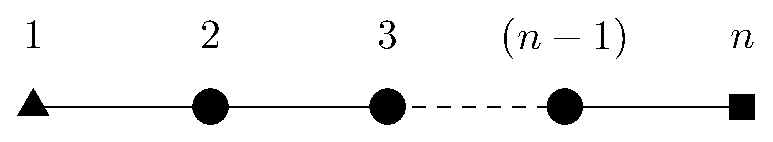
\includegraphics [scale=0.8] {images/1d}
    \caption{Область решения одномерной задачи теплопроводности.} 
    \label{images:1d}  
\end{figure}

Система линейных уравнений для МКЭ в матричной форме:

\begin{equation}
    K \overline{\psi} = \overline{b}
    \label{equ:slau}  
\end{equation}

где $K$ - матрица жесткости, $ \overline{\psi}$ - вектор неизвестных ячейковых температур в узлах, $ \overline{b}$ - вектор правой части.
Матрица жесткости имеет вид:

\begin{equation}
    K =
    \left(
        \begin{array}{cccccc}
            k_{1,1} & k_{1,2} & 0       & \ldots & 0           & 0         \\
            k_{2,1} & k_{2,2} & k_{2,3} & \ldots & 0           & 0         \\
            0       & k_{3,2} & k_{3,3} & \ldots & 0           & 0         \\
            \vdots  & \vdots  & \vdots  &        & \vdots      & \vdots    \\
            0       & 0       & 0       & \ldots & k_{n-1,n-1} & k_{n-1,n} \\
            0       & 0       & 0       & \ldots & k_{n,n-1}   & k_{n,n}   \\
        \end{array}
    \right)
    \label{equ:k1}  
\end{equation}

Коэффициенты $k_{1,2}$ и $k_{2,1}$ отражают взаимосвязь узлов $1$ и $2$, лежащих в пределах одного конечного эдементы, они не равны нулю. 
Коэффициенты $k_{1,n-1}$ и $k_{n-1,1}$ равны нулю, так как узлы $1$ и $n-1$ в разных конечных элементах. 
В матрице жесткости производятся следующие замены:

% \begin{equation}
%         \begin{array}{c}
%             k_{1,n-1} \leftarrow k_{n,n-1}, \\
%             k_{n-1,1} \leftarrow k_{n-1,N}, \\
%             k_{n,n-1} \leftarrow 0, \\
%             k_{n-1,n} \leftarrow 0, \\
%             k_{n,n}   \leftarrow 1
%         \end{array}
% \end{equation}

% \begin{equation}
        \begin{align*}
            k_{1,n-1} &\leftarrow k_{n,n-1}, \\
            k_{n-1,1} &\leftarrow k_{n-1,N}, \\
            k_{n,n-1} &\leftarrow 0, \\
            k_{n-1,n} &\leftarrow 0, \\
            k_{n,n}   &\leftarrow 1
        \end{align*}
% \end{equation}

получим матрицу такого вида:

\begin{equation}
    K^* =
    \left(
        \begin{array}{cccccc}
            k_{1,1}   & k_{1,2} & 0       & \ldots & k_{1,n-1}   & 0      \\
            k_{2,1}   & k_{2,2} & k_{2,3} & \ldots & 0           & 0      \\
            0         & k_{3,2} & k_{3,3} & \ldots & 0           & 0      \\
            \vdots    & \vdots  & \vdots  &        & \vdots      & \vdots \\
            k_{n-1,1} & 0       & 0       & \ldots & k_{n-1,n-1} & 0      \\
            0         & 0       & 0       & \ldots & 0           & 1      \\
        \end{array}
    \right)
    \label{equ:k2}  
\end{equation}

Вектор правой части остаётся неизменным.

Полученое уравнение (\ref{eq:new_K}) условно соответствует области решения в виде <<кольца>> (рис. \ref{images:1d_loop}).

\begin{equation}
    K^* \overline{\psi^*} = \overline{b}
    \label{eq:new_K}  
\end{equation}

\begin{figure} [ht]
    \center
    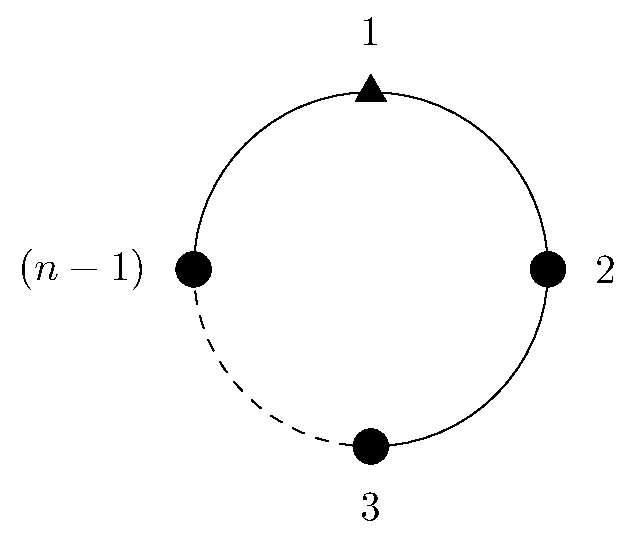
\includegraphics [scale=0.8] {images/1d_loop}
    \caption{Области решения в виде <<кольца>>.} 
    \label{images:1d_loop}  
\end{figure}

После решения уравнения (\ref{eq:new_K}) производится обратная замена в векторе $\overline{\psi^*}$, что бы вернуть <<выброшенный>> граничный узел. 
Само решение получается с точностью до константы и на него налагается дополнительное условние, именуемое нормировки:

\begin{equation}
    \left< \Psi \right> = 0
\end{equation}

После нормировки решения $ \overline{\psi^*} $ получается $ \overline{\psi} $ , являющееся решение исходной системы уравнений \ref{equ:slau}. 

\textbf{Пример для случая 2-переодического композитного материала.} 
Задача имеет аналогичный вид задаче (\ref{equ:1d_beg})-(\ref{periodic_cell}) с той разницей что она поставленна для двумерной области решения. 
Пример сетки конечных элементов для двумерной ячейки периодичности представлен на рис. \ref{image:2d}.
Область разбита на четырёхугольные конечные элементы. 
Разбиение может иметь самый произвольный характер, за исключением граничных точек.
Граничные узлы должны быть расположенны симметрично, отночительно вертикальной и горизонтальной осей, проходящих через центр области.
Это означает что координаты $\xi_x$ узлов на левой грани должны совпадать с координатами $\xi_x$ аналогичных узлов правой грани.
То же для верхней и нижней граней, совпадение по координатам $\xi_y$.
На примере (рис.\ref{image:2d}) граничные узла расположенны равномерно, с постоянным шагом, но могут быть расположены и неравномерно.

\begin{figure} [ht] 
    \center
    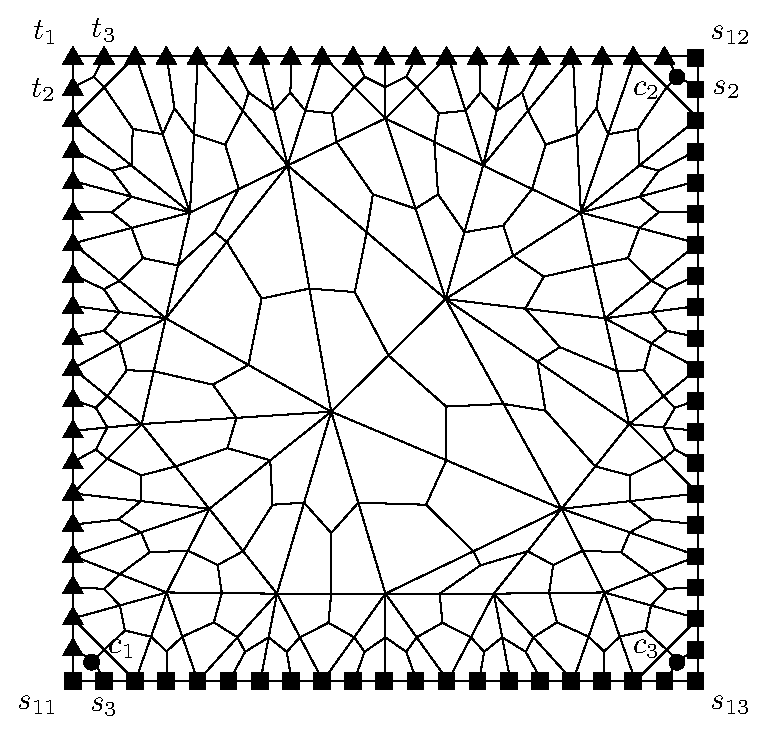
\includegraphics [scale=0.8] {images/2d}
    \caption{Область решения двумерной задачи теплопроводности.} 
    \label{images:2d}  
\end{figure}

С матрицей жесткости выполняются манипуляции аналогичные манипуляциям (\ref{equ:k1})-(\ref{equ:k2}), <<заменяются>> узлы, отмеченные квадратами (буква <<s>>),
на узлы, отмеченные треуголниками (буква <<t>>). Внутренние узлы на рис. \ref{image:2d} отмечены только в трёх точках, чтол бы не забивать изображение, и символьно обозначены буквами <<c>>.
Пример замены коэффициентов:

% \begin{equation}
%         \begin{array}{ccccc}
%             k_{t_1,c_1} = k_{s_{11},c_1},  k_{t_1,c_2} = k_{s_{12},c_2},  k_{t_1,c_3} = k_{s_{13},c_3},  k_{t_2,c_2} = k_{s_2,c_2},  k_{t_3,c_1} = k_{s_3,c_1}, \\
%             k_{s_{11},c_1} = 0,  k_{s_{12},c_2} = 0,  k_{s_{13},c_3} = 0,  k_{s_2,c_2} = 0,  k_{s_3,c_1} = 0, \\
%             k_{s_{11},s_{11}} = 1,  k_{s_{12},s_{12}} = 1,  k_{s_{13},s_{13}} = 1,  k_{s_2,s_2} = 1,  k_{s_3,s_3} = 1
%         \end{array}
% \end{equation}

\begin{align*}
    k_{t_1,c_1} &\leftarrow k_{s_{11},c_1}, & k_{t_1,c_2} &\leftarrow k_{s_{12},c_2}, & k_{t_1,c_3} &\leftarrow k_{s_{13},c_3}, & k_{t_2,c_2} &\leftarrow k_{s_2,c_2}, & k_{t_3,c_1} &\leftarrow k_{s_3,c_1}, \\
    k_{s_{11},c_1} &\leftarrow 0, & k_{s_{12},c_2} &\leftarrow 0, & k_{s_{13},c_3} &\leftarrow 0, & k_{s_2,c_2} &\leftarrow 0, & k_{s_3,c_1} &\leftarrow 0, \\
    k_{s_{11},s_{11}} &\leftarrow 1, & k_{s_{12},s_{12}} &\leftarrow 1, & k_{s_{13},s_{13}} &\leftarrow 1, & k_{s_2,s_2} &\leftarrow 1, & k_{s_3,s_3} &\leftarrow 1
\end{align*}

Замены для двумерной области решения в целом аналогичны заменам в одномерной, но есть особенность в угловых точках. 
Один уголовой узел $t_1$ <<заменяет>> все три остальных угловых узла: $s_{11}$, $s_{12}$, $s_{13}$.
После проведённых замен область решения станет соответствовать <<тору>>.

\textbf{Пример для случая 3-переодического композитного материала.} 
Задача имеет аналогичный вид задаче (\ref{equ:1d_beg})-(\ref{periodic_cell}) с той разницей что она поставленна для трёхмерной области решения. 
Пример сетки конечных элементов для двумерной ячейки периодичности представлен на рис. \ref{image:3d}.
Изображение плохо демонстрирует сетку, но не представляется возможным адекватно отобразить трёхмерную область на плоскость.
Область разбита на шестигранные объёмные конечные элементы. 
Разбиение может иметь самый произвольный характер, за исключением граничных точек.
Граничные узлы должны быть расположенны симметрично, отночительно трёх осей, проходящих через центр области.
Это означает что координаты $(\xi_x, \xi_y)$ узлов на одной грани должны совпадать с координатами $(\xi_x, \xi_y)$ аналогичных узлов на противоположной грани.
То же правило для двух остальных пар граней, с координатами $(\xi_x, \xi_z)$ и $(\xi_y, \xi_z)$.

\begin{figure} [ht] 
    \center
    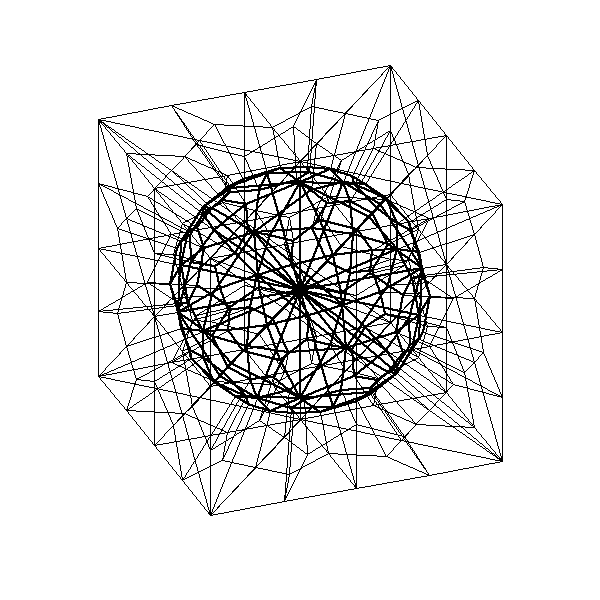
\includegraphics [scale=0.8] {images/3d}
    \caption{Область решения трёхмерной задачи теплопроводности.} 
    \label{images:3d}  
\end{figure}

С матрицей жесткости выполняются манипуляции аналогичные манипуляциям (\ref{equ:k1})-(\ref{equ:k2}).
Имеются особенности в угловый узлах и узлах на гранях. 
Один уголовой узел <<заменяет>> пять остальных угловых узлов. 
Узлы одного ребра заменяют соответствующие узлы остальных трёх рёбер, расположенных вдоль той же оси координат.


% \begin{equation*}
%     \left(
%         \begin{array}{*{13}c}
%              & \textcolor{blue}{B_1} & \ldots & \textcolor{blue}{B_2} & \ldots & \textcolor{red}{R_1} & \ldots & \textcolor{red}{R_2} & \ldots & D_1 & \ldots & D_2 & \ldots \\
%             \textcolor{blue}{B_1} & k_{B_1B_1} &  & k_{B_1B_2} &  & 0 &  & 0 &  & k_{R_1D_1} &  & k_{R_1D_2} &  \\
%             \vdots &  &  &  &  &  &  &  &  &  &  &  &  \\
%             \textcolor{blue}{B_2} & k_{B_1B_2} &  & k_{B_2B_2} &  & 0 &  & 0 &  & k_{R_2D_1} &  & k_{R_2D_2} &  \\
%             \vdots &  &  &  &  &  &  &  &  &  &  &  &  \\
%             \textcolor{red}{R_1} & 0 &  & 0 &  & 1 &  & 0 &  & 0 &  & 0 &  \\
%             \vdots &  &  &  &  &  &  &  &  &  &  &  &  \\
%             \textcolor{red}{R_2} & 0 &  & 0 &  & 0 &  & 1 &  & 0 &  & 0 &  \\
%             \vdots &  &  &  &  &  &  &  &  &  &  &  &  \\
%             D_1 & k_{R_1D_1} &  & k_{R_2D_1} &  & 0 &  & 0 &  & k_{D_1D_1} &  & k_{D_1D_2} &  \\
%             \vdots &  &  &  &  &  &  &  &  &  &  &  &  \\
%             D_2 & k_{R_1D_2} &  & k_{R_2D_2} &  & 0 &  & 0 &  & k_{D_1D_2} &  & k_{D_2D_2} &  \\
%             \vdots &  &  &  &  &  &  &  &  &  &  &  &  \\
%         \end{array}
%     \right)
% \end{equation*}


\section{Правая часть}\label{sec:ch2/sec2}

\section{Преобразование коэффициентов}\label{sec:ch2/sec3}

\section{Решение системы уравнений}\label{sec:ch2/sec4}

\clearpage
           % Глава 2
\chapter{Практические результыты}\label{ch:ch3}

\section{Макротеплопроводность волокнистого материала}\label{ch:ch3/sect1}

\section{Упругие макрохарактеристики волокнистого материала}\label{ch:ch3/sect2}

\section{Упругие макрохарактеристики материала армированного периодическими решетками}\label{ch:ch3/sect3}

\section{Напряженное состояние в волокнистом материале вблизи отверстия}\label{ch:ch3/sect4}

\section{Температурное поле в обжимном кольце}\label{ch:ch3/sect5}

\clearpage
           % Глава 3
\chapter{Эксперименты}\label{ch:ch4}

\section{Хз получится ли}\label{ch:ch3/sect1}


\clearpage
           % Глава 4
\include{Dissertation/conclusion}      % Заключение
\chapter*{Список сокращений и условных обозначений} % Заголовок
\addcontentsline{toc}{chapter}{Список сокращений и условных обозначений}  % Добавляем его в оглавление
\noindent
%\begin{longtabu} to \dimexpr \textwidth-5\tabcolsep {r X}
\begin{longtabu} to \textwidth {r X}
% Жирное начертание для математических символов может иметь
% дополнительный смысл, поэтому они приводятся как в тексте
% диссертации

\textbf{МКЭ} & метод конечных элементов\\


\end{longtabu}
\addtocounter{table}{-1}% Нужно откатить на единицу счетчик номеров таблиц, так как предыдующая таблица сделана для удобства представления информации по ГОСТ
        % Список сокращений и условных обозначений
\include{Dissertation/dictionary}      % Словарь терминов
\include{Dissertation/references}      % Список литературы
\include{Dissertation/lists}           % Списки таблиц и изображений (иллюстративный материал)

%%% Настройки для приложений
\appendix
% Оформление заголовков приложений ближе к ГОСТ:
\setlength{\midchapskip}{20pt}
\renewcommand*{\afterchapternum}{\par\nobreak\vskip \midchapskip}
\renewcommand\thechapter{\Asbuk{chapter}} % Чтобы приложения русскими буквами нумеровались

\chapter{Примеры вставки листингов программного кода}\label{app:A}

Для крупных листингов есть два способа. Первый красивый, но в нём могут быть
проблемы с поддержкой кириллицы (у вас может встречаться в~комментариях
и печатаемых сообщениях), он представлен на листинге~\ref{lst:hwbeauty}.
\begin{ListingEnv}[!h]% настройки floating аналогичны окружению figure
    \captiondelim{ } % разделитель идентификатора с номером от наименования
    \caption{Программа ,,Hello, world`` на \protect\cpp}\label{lst:hwbeauty}
    % окружение учитывает пробелы и табуляции и применяет их в сответсвии с настройками
    \begin{lstlisting}[language={[ISO]C++}]
	#include <iostream>
	using namespace std;

	int main() //кириллица в комментариях при xelatex и lualatex имеет проблемы с пробелами
	{
		cout << "Hello, world" << endl; //latin letters in commentaries
		system("pause");
		return 0;
	}
    \end{lstlisting}
\end{ListingEnv}%
Второй не~такой красивый, но без ограничений (см.~листинг~\ref{lst:hwplain}).
\begin{ListingEnv}[!h]
    \captiondelim{ } % разделитель идентификатора с номером от наименования
    \caption{Программа ,,Hello, world`` без подсветки}\label{lst:hwplain}
    \begin{Verb}

        #include <iostream>
        using namespace std;

        int main() //кириллица в комментариях
        {
            cout << "Привет, мир" << endl;
        }
    \end{Verb}
\end{ListingEnv}

Можно использовать первый для вставки небольших фрагментов
внутри текста, а второй для вставки полного
кода в приложении, если таковое имеется.

Если нужно вставить совсем короткий пример кода (одна или две строки),
то~выделение  линейками и нумерация может смотреться чересчур громоздко.
В таких случаях можно использовать окружения \texttt{lstlisting} или
\texttt{Verb} без \texttt{ListingEnv}. Приведём такой пример
с указанием языка программирования, отличного от~заданного по умолчанию:
\begin{lstlisting}[language=Haskell]
fibs = 0 : 1 : zipWith (+) fibs (tail fibs)
\end{lstlisting}
Такое решение~--- со вставкой нумерованных листингов покрупнее
и вставок без выделения для маленьких фрагментов~--- выбрано,
например, в книге Эндрю Таненбаума и Тодда Остина по архитектуре
%компьютера~\autocite{TanAus2013} (см.~рис.~\ref{fig:tan-aus}).

Наконец, для оформления идентификаторов внутри строк
(функция \lstinline{main} и~тому подобное) используется
\texttt{lstinline} или, самое простое, моноширинный текст
(\texttt{\textbackslash texttt}).

Пример~\ref{lst:internal3}, иллюстрирующий подключение переопределённого
языка. Может быть полезным, если подсветка кода работает криво. Без
дополнительного окружения, с подписью и ссылкой, реализованной встроенным
средством.
\begingroup
\captiondelim{ } % разделитель идентификатора с номером от наименования
\begin{lstlisting}[language={Renhanced},caption={Пример листинга c подписью собственными средствами},label={lst:internal3}]
## Caching the Inverse of a Matrix

## Matrix inversion is usually a costly computation and there may be some
## benefit to caching the inverse of a matrix rather than compute it repeatedly
## This is a pair of functions that cache the inverse of a matrix.

## makeCacheMatrix creates a special "matrix" object that can cache its inverse

makeCacheMatrix <- function(x = matrix()) {#кириллица в комментариях при xelatex и lualatex имеет проблемы с пробелами
    i <- NULL
    set <- function(y) {
        x <<- y
        i <<- NULL
    }
    get <- function() x
    setSolved <- function(solve) i <<- solve
    getSolved <- function() i
    list(set = set, get = get,
    setSolved = setSolved,
    getSolved = getSolved)

}


## cacheSolve computes the inverse of the special "matrix" returned by
## makeCacheMatrix above. If the inverse has already been calculated (and the
## matrix has not changed), then the cachesolve should retrieve the inverse from
## the cache.

cacheSolve <- function(x, ...) {
    ## Return a matrix that is the inverse of 'x'
    i <- x$getSolved()
    if(!is.null(i)) {
        message("getting cached data")
        return(i)
    }
    data <- x$get()
    i <- solve(data, ...)
    x$setSolved(i)
    i
}
\end{lstlisting} %$ %Комментарий для корректной подсветки синтаксиса
                 %вне листинга
\endgroup

Листинг~\ref{lst:external1} подгружается из внешнего файла. Приходится
загружать без окружения дополнительного. Иначе по страницам не переносится.
\begingroup
\captiondelim{ } % разделитель идентификатора с номером от наименования
    \lstinputlisting[lastline=78,language={R},caption={Листинг из внешнего файла},label={lst:external1}]{listings/run_analysis.R}
\endgroup

        % Приложения

\end{document}
